\section{Data Analysis}
The following section will include an overview and visualisation of the data acquired for the research, and how it was processed for use in the neural networks.

\subsection{Engine Health Monitoring Data} \label{sec:ehm}
The research was carried out on \ac{ehm} data. This data was recorded by sensors in 231 BR725 engines during a total of 14\,045 flights, and returned on a voluntary basis to Rolls-Royce by operators for analysis.

The BR725 is used in the Gulfstream G650, a business jet built for up to 18 passengers. Each G650 has two engines; to minimise the amount of data used, the values used in this thesis were taken from the left engine only.

\begin{figure}
    \centering
    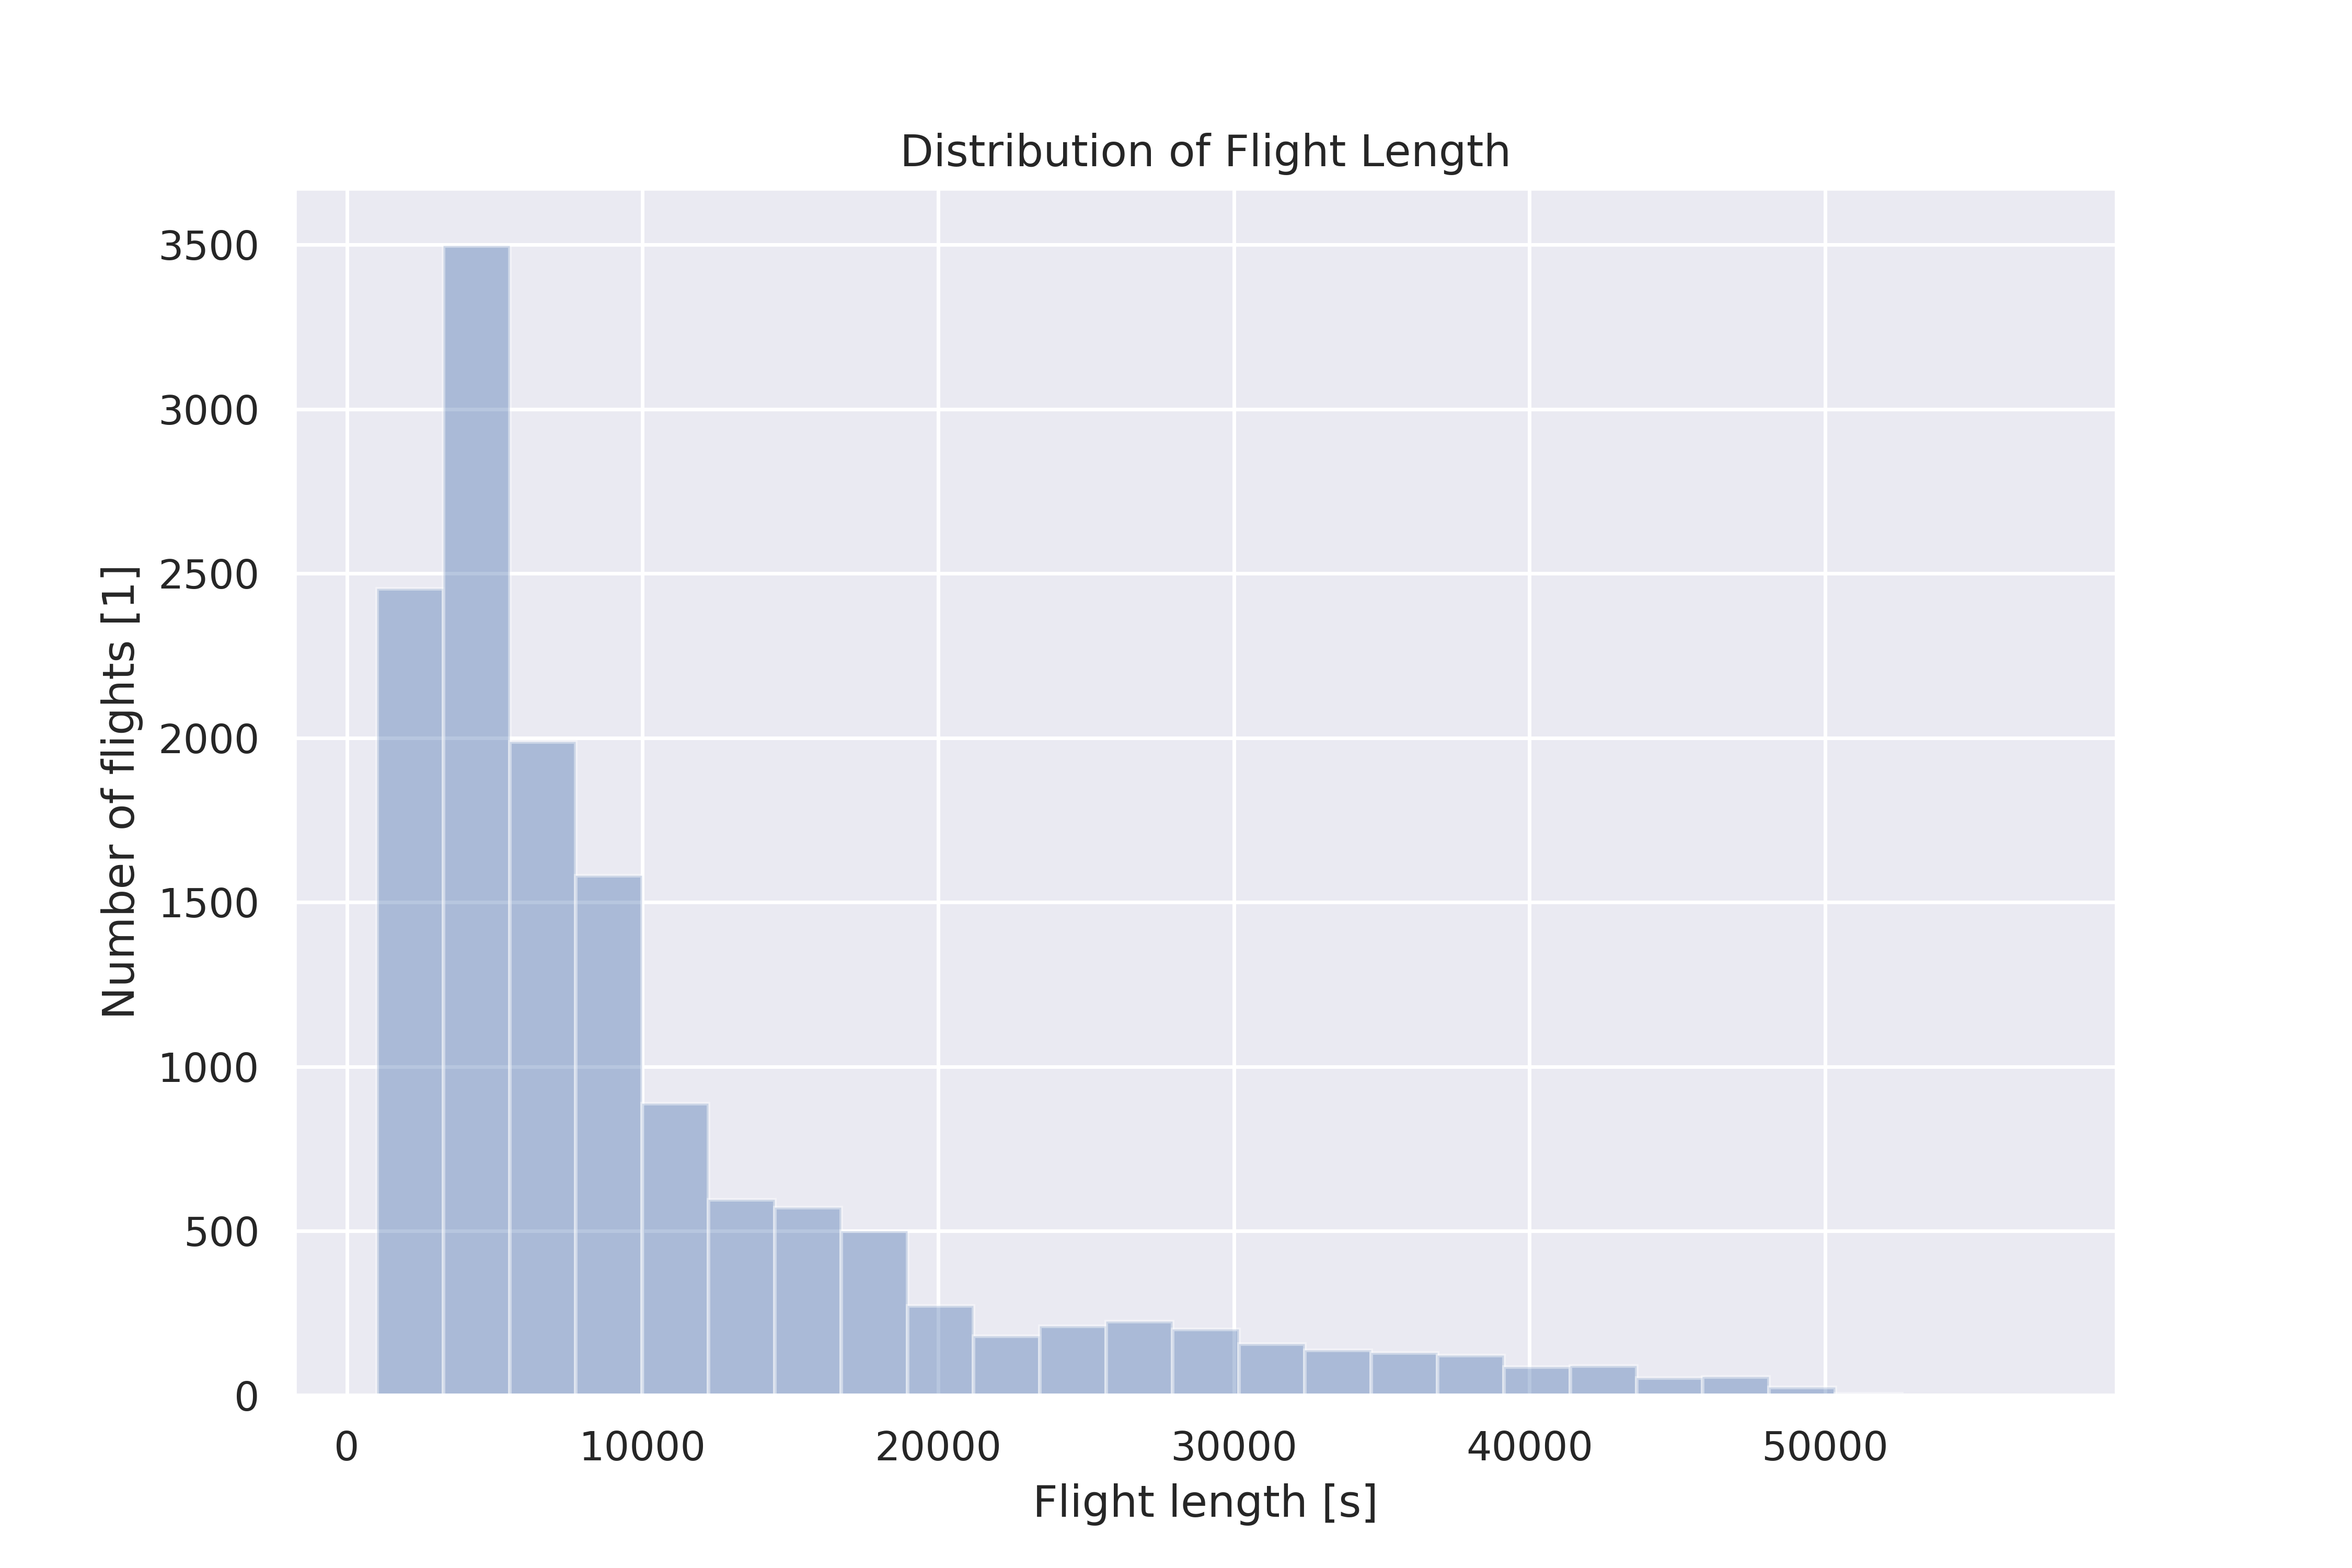
\includegraphics[width=\textwidth]{length_hist}
    \caption{\label{fig:flight_len} A histogram of the lengths of 14\,045 flights}
\end{figure}

The flights range in length from 1\,013 to 57\,062 seconds (approximately 0.28 to 15.85 hours), with a mean length of 10\,182.82 seconds and a standard deviation of 9\,561.03 seconds (see Figure \ref{fig:flight_len}).

Each flight is summarised in a CSV file with 216 columns, comprising one timestamp and 215 values for each second of recording time.

\begin{figure}
    \centering
    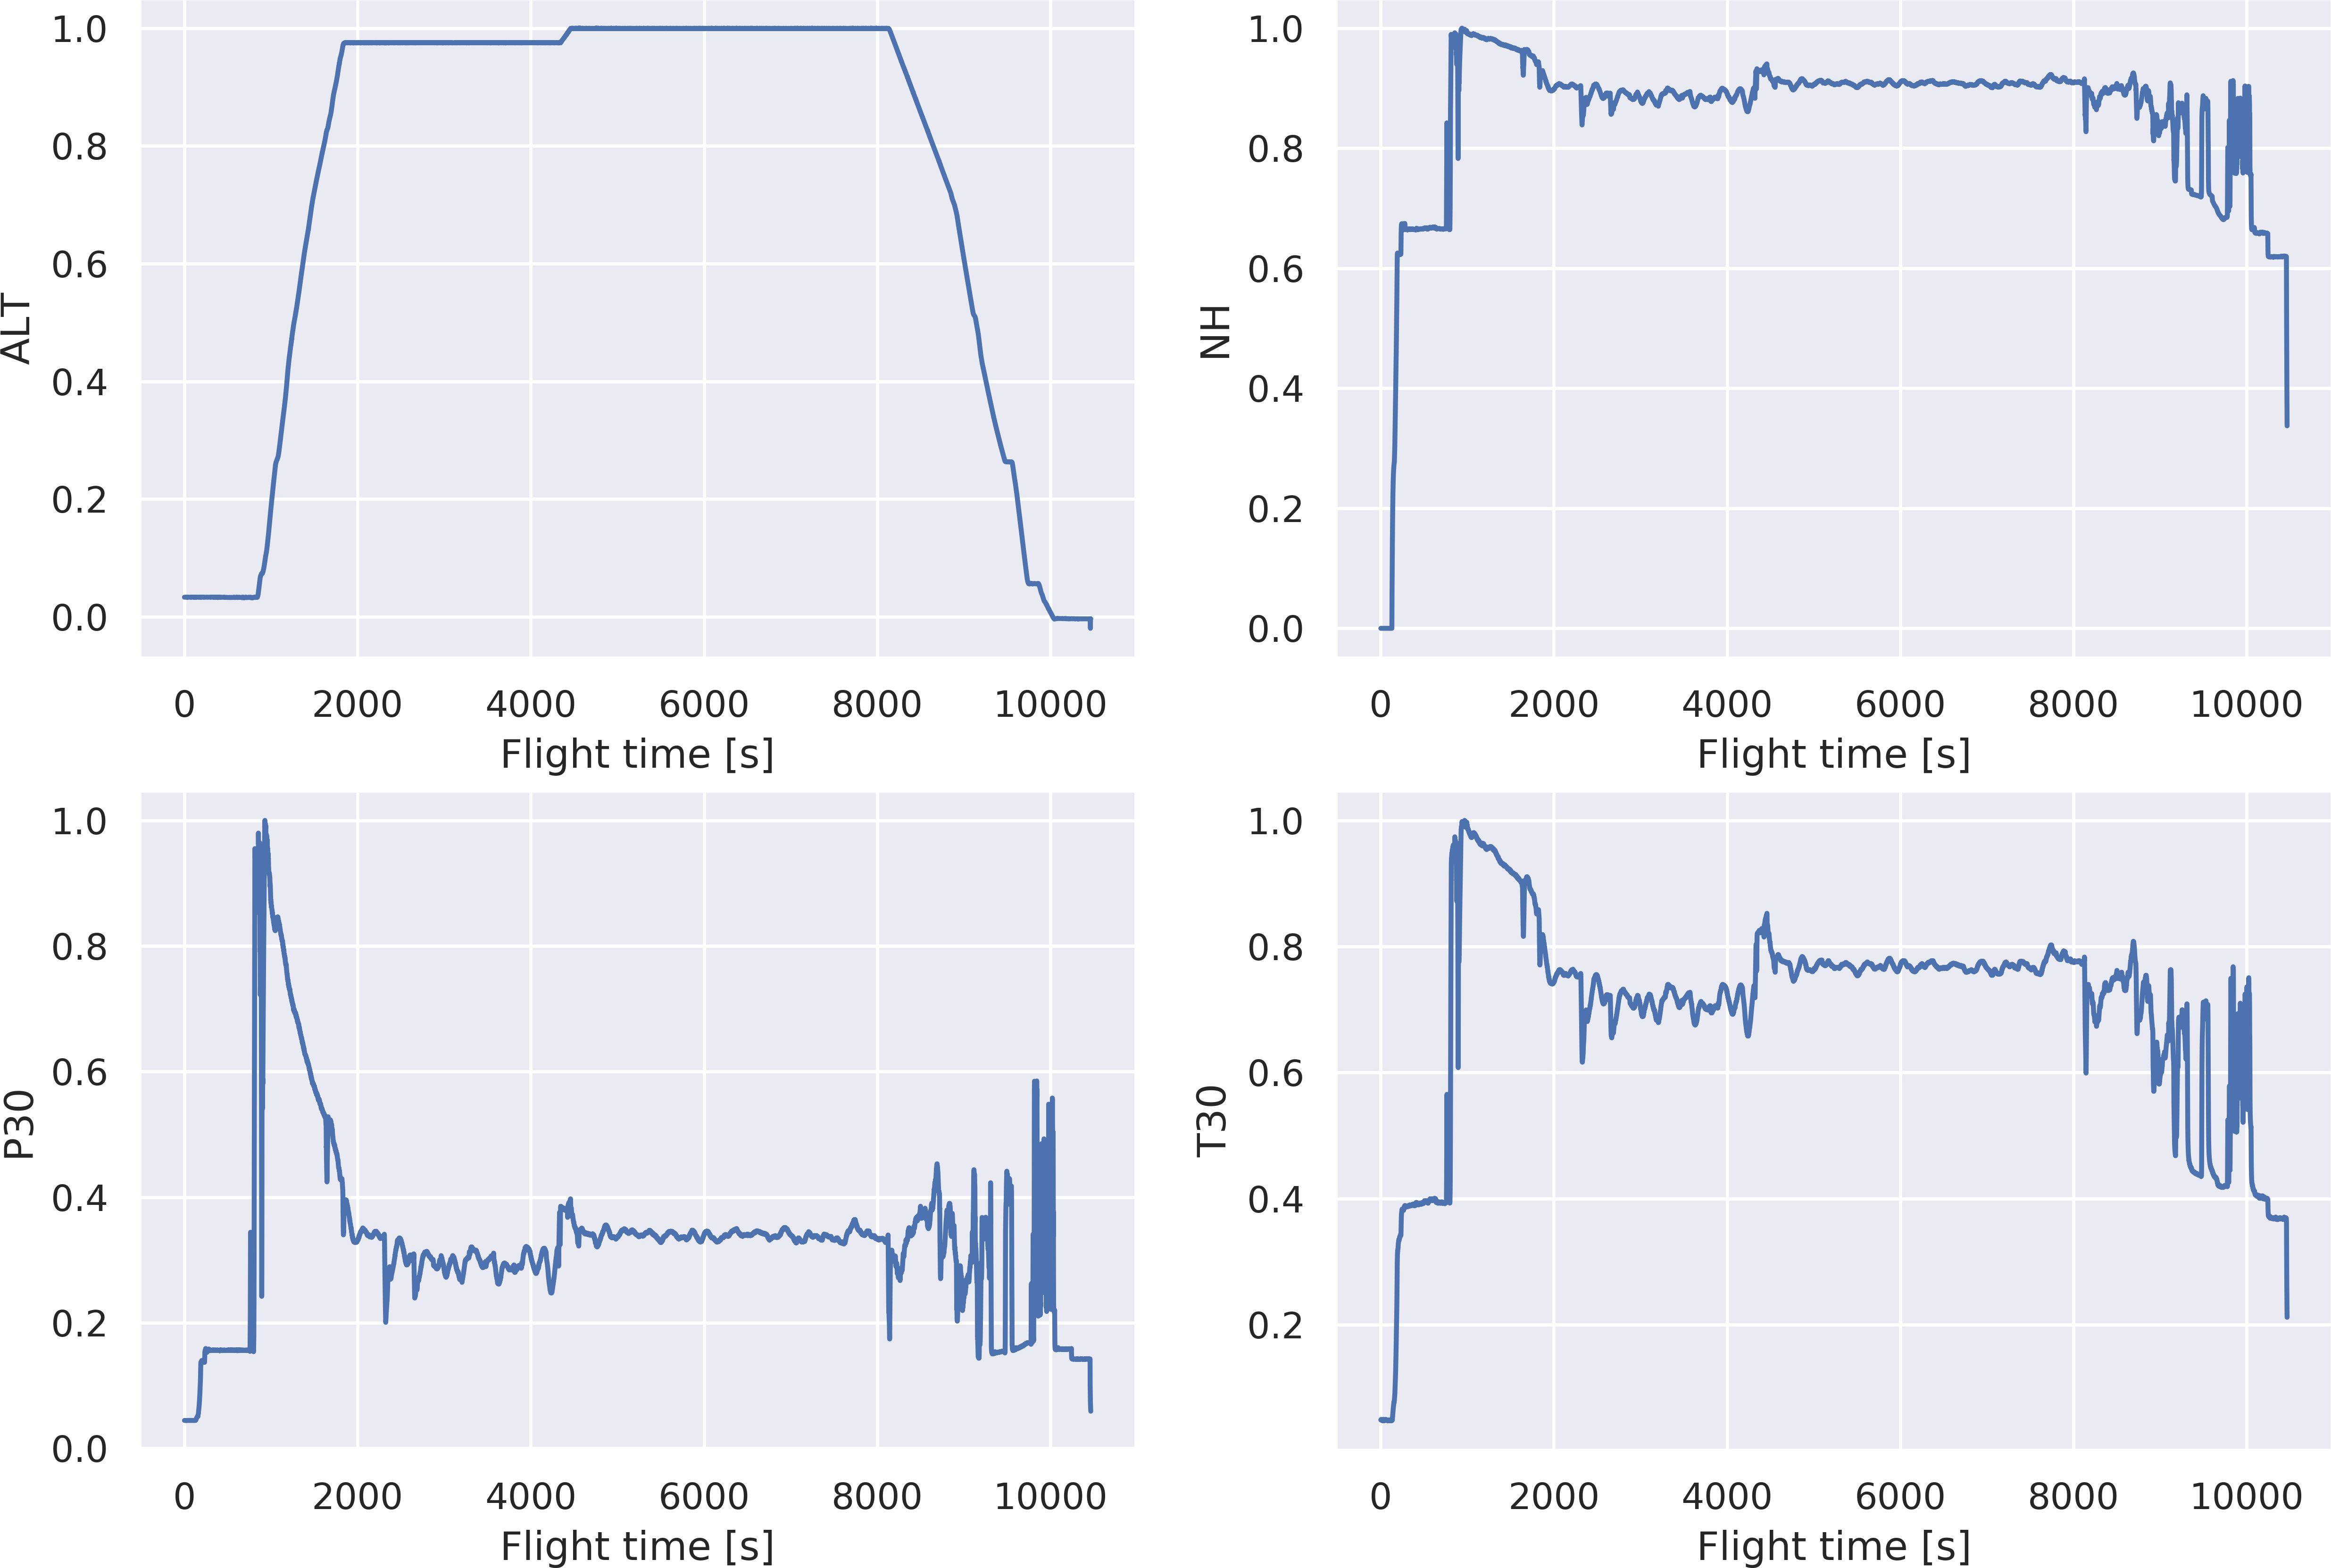
\includegraphics[width=\textwidth]{0815}
    \caption{\label{fig:flight_example} ALT, NH, P30 and T30 of a randomly selected flight, Flight 0815. All parameter values normalised.}
\end{figure}

The four flight parameters extracted from these \ac{csv} files were altitude (ALT), rotational speed of the high-pressure shaft (NH), and pressure and temperature of air exiting the compressor (P30 and T30, respectively). These values are shown (normalised) for one randomly selected flight, hereinafter referred to as \textit{Flight 0815}, in Figure \ref{fig:flight_example}.

NH is measured in rotations per minute, and recorded as a percentage of the maximum rotational speed defined for the engine. It therefore takes any value between 0 and 100. ALT is measured in feet; the maximum altitude across all flights was 51\,148 feet, or 15\,590 metres. P30 is measured in PSIA, and ranges between 5.3 and 385.8 across all flights. The units of T30 are degrees Celsius and the values range from -12.0\textdegree{C} to 590.5\textdegree{C}.

\subsection{Flight Phases} \label{sec:phases}
A flight can be split into several phases: preflight, taxi out, take-off, climb, cruise, descent, reverse thrust and taxi in. These phases were extracted using internal Rolls-Royce software \cite[]{konig_br725stats_2018} that combined the flight mode parameter from \ac{ehm} data \cite[]{reischl_br700-725a1-12_2014} and custom conditions for optimisation. The conditions are summarised in table \ref{tab:flight_phases}.

The \ac{fm} often makes use of the parameter \ac{wow}, a boolean parameter with a value of 1 if the aircraft's weight is supported by its wheels, otherwise 0. Other parameters used for determining \ac{fm} include ground speed, intertial vertical speed, wing flap angle and \ac{tra}.

\begin{table}
    \begin{center}
        \caption{\label{tab:flight_phases} Summary of flight phases, corresponding lengths after downsampling (Section \ref{sec:downsample}), and conditions at which they begin \cite[]{konig_br725stats_2018}. \ac{fm} conditions in accordance with \citet{reischl_br700-725a1-12_2014}.}
        \begin{tabular}{ l c l }
            Phase & Downsampled & Conditions \\ & length & \\
            \midrule
            Preflight & 1 & \ac{fm} \(= 2\) \\
            Taxi out & 5 & left or right engine is switched on \\
            Take-off & 10 & \ac{fm} \(= 4\) \\
            % & \ac{wow} \(= 1\) \\
            % & \ac{tra} \(> 20^{\circ}\) for both engines \\
            % & ground speed \(> 28\) knots \\
            Climb & 20 & \ac{wow} \(= 0\) \\
            & & intertial vertical speed \(> 500\) \(\text{ft} / \text{min}\) \\
            & & altitude at least \(1500 \) m greater than at take-off \\
            Cruise & 20 & \ac{fm} \(= 6\) \\
            & & altitude greater than 85\% of maximum altitude \\
            Descent & 10 & \ac{fm} \(= 7\) or \ac{fm} \(= 8\) \\
            & & \ac{tra} \(< 20^{\circ} \) for both engines \\
            & & Time to destination \(< 45\) \(\text{min}\) \\
            Reverse thrust & 10 & \ac{fm} \(= 9\) \\
            Taxi in & 5 & reverse thrust phase ended
        \end{tabular}
    \end{center}
\end{table}

\begin{figure}
    \centering
    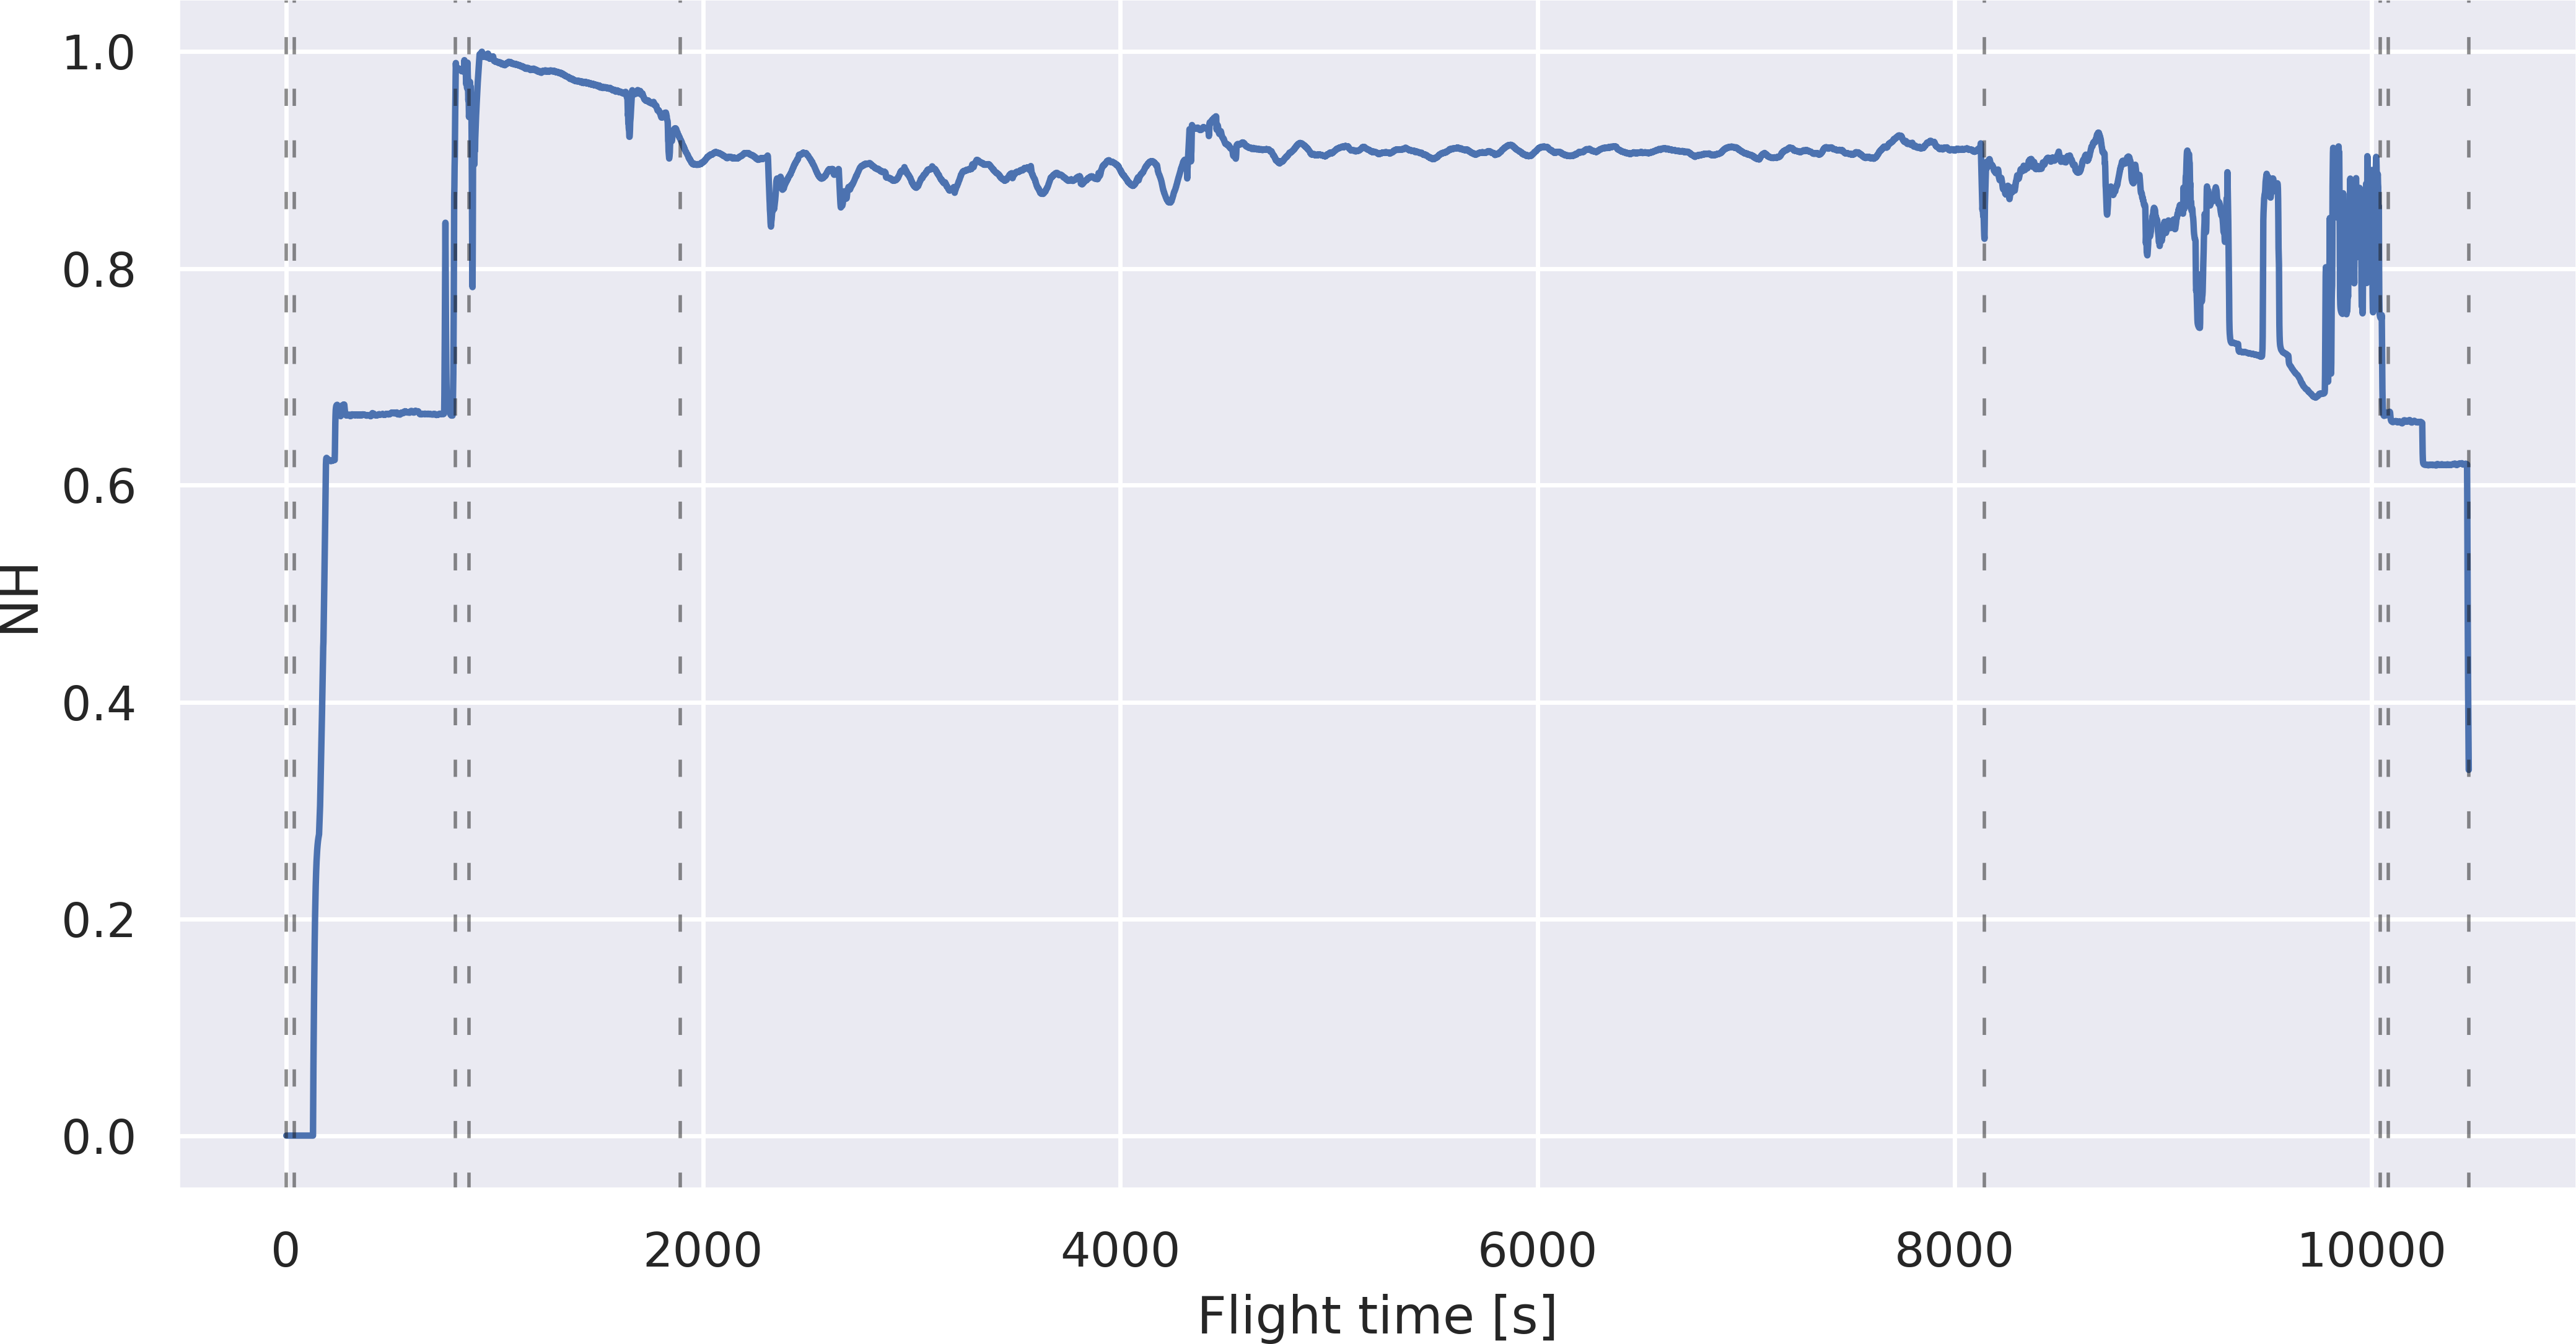
\includegraphics[width=\textwidth]{6008_20150409074414_NH_phases}
    \caption{\label{fig:phases_example} Phase boundaries of NH indicated on Flight 0815}
\end{figure}

Figure \ref{fig:phases_example} shows the NH plot from Flight 0815; dashed vertical lines represent phase boundaries.

\subsection{Features} \label{sec:features}
Seven features of the \ac{hpt} disk were selected as points of interest for the research (see locations in Figure \ref{fig:hpt1}). The features were selected as critical points on the disk at which damage was expected to be highest, based on stress curves from previously computed \ac{fe} models. The seven features included three pairs with similar stress curves and resulting damage values: features 1 and 2 are both located in the bore; 4 and 5 are located under the front and rear drive arms, respectively; 6 and 7 are thermally sensitive features located in a seal fin and an air hole, respectively.

\begin{figure}
    \centering
    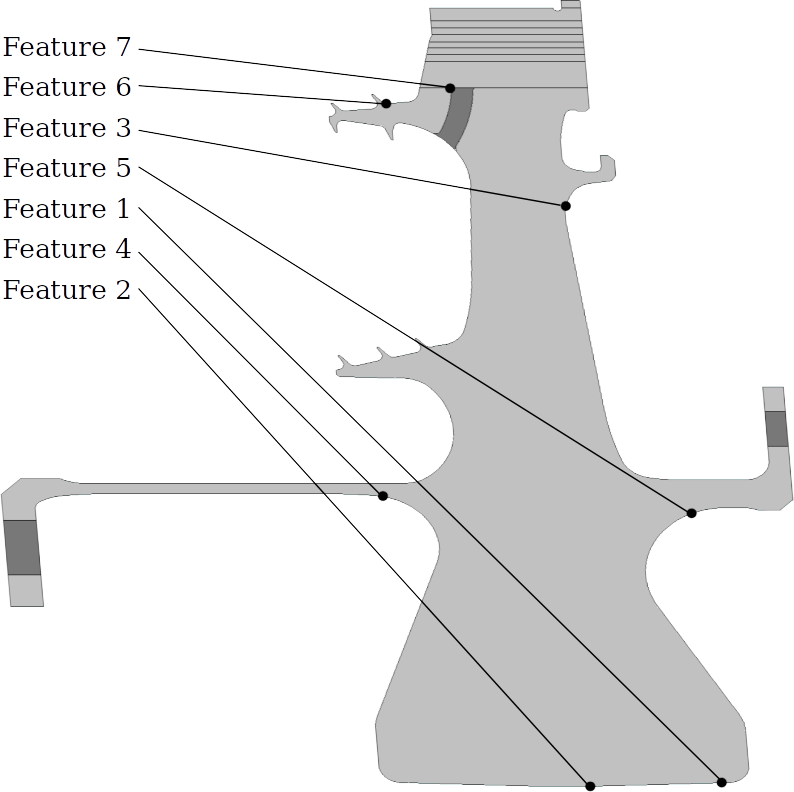
\includegraphics[width=0.5\textwidth]{hpt1_draw}
    \caption{\label{fig:hpt1} Location of features 1 to 7 on a cross-section of the \ac{hpt} disk. (The disk was scaled and sheared to protect intellectual property.)}
\end{figure}

The features were selected in pairs to investigate the possibility of using a small number of damage values from various locations on the disk to predict damage in others, in case models based on flight data alone turned out not to be feasible.

Due to their location within the bore with no direct contact to the hot, pressurised air, features 1 and 2 are not expected to be sensitive to temperature or pressure. Therefore, changes in these parameters during the flight should not influence damage in these features. Rotational speed should have the greatest effect on these features.

Features 4 and 5, on the other hand, are expected to be sensitive to pressure due to their contact with high-pressure air, but not to temperature due to a lack of direct contact with hot air from the combustion chamber. Features 6 and 7, critical points with direct contact to the hot air, are expected to be highly sensitive to temperature.

\subsection{Cycle Counter} \label{sec:cyclecounter}
The \ac{ehm} data was processed using the company's internal Cycle Counter software to determine the number of cycles consumed by each feature during each flight. Figures \ref{fig:dmg_dist_low} and \ref{fig:dmg_dist_high} show the distribution of damage data (98\,315 values across 7 features from 14\,045 flights) computed by the Cycle Counter. For clarity in illustration and comparison, the distributions were split at a damage of 2.0 cycles: Figure \ref{fig:dmg_dist_low} contains all damage values between 0 and 2 cycles, with the overwhelming majority of the values (97\,868, 99.5\%) falling within this range; Figure \ref{fig:dmg_dist_high} contains all values above 2 cycles (with a maximum damage of 14.1 cycles), containing only 447 data points, or 0.05\%, of the total.

\begin{figure}
    \centering
    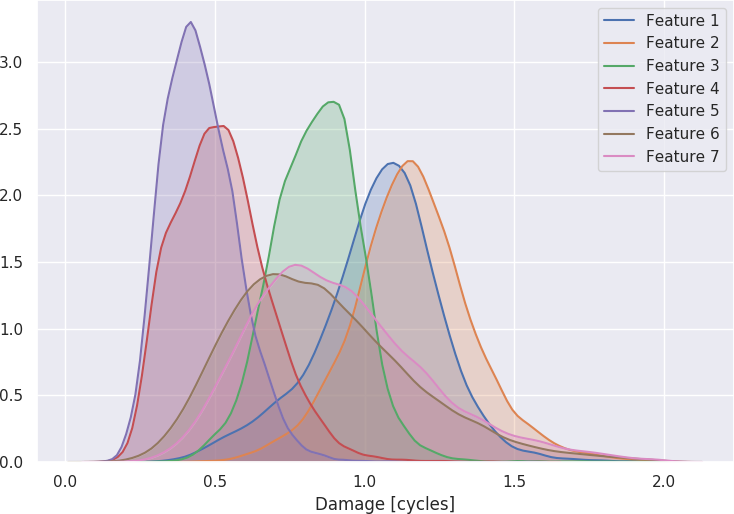
\includegraphics[width=\textwidth]{distribution_low_2}
    \caption{\label{fig:dmg_dist_low} \ac{kde} plot displaying the distribution of damage cycles consumed by the seven features over 99.5\% of all 14\,045 flights (with damage of up to two cycles)}
\end{figure}

It should be noted that, in Figure \ref{fig:dmg_dist_low}, there are clear pairwise similarities in the distributions of the pairs mentioned in Section \ref{sec:features}. This is of no surprise, but could be highly valuable if a supervised machine learning model can be trained to extrapolate this (and other) information to further features.

\begin{figure}
    \centering
    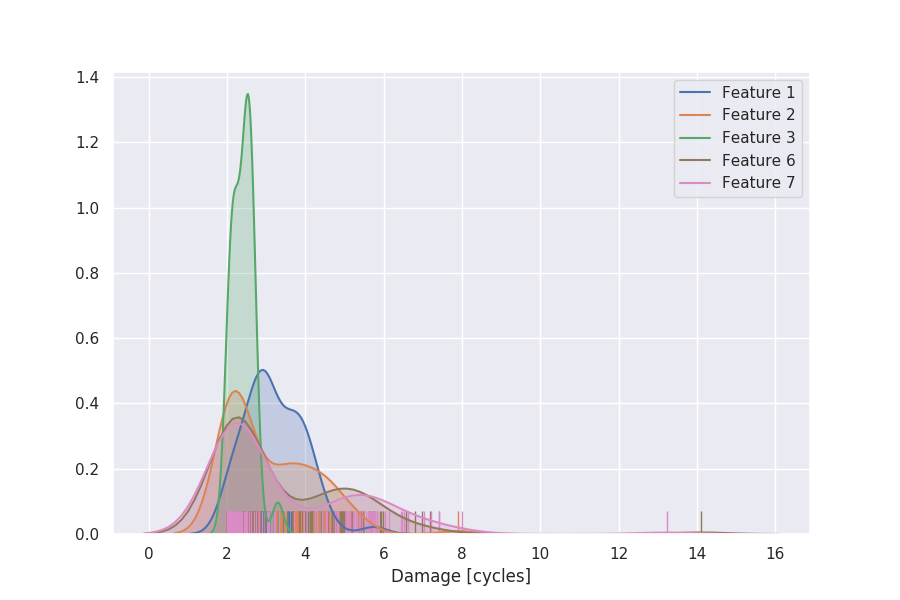
\includegraphics[width=\textwidth]{distribution_high_2}
    \caption{\label{fig:dmg_dist_high} \ac{kde} plot displaying the distribution of damage cycles consumed by the seven features over 0.5\% of all 14\,045 flights (with damage of two cycles and above). The short vertical lines at the base represent individual data points. No flight caused damage of more than 2 cycles in features 4 and 5.}
\end{figure}

\subsection{Time Series Approximation} \label{sec:downsample}
The input layer of an \ac{mlp} requires a fixed number of input values in order to be able to train weights and biases. As shown in Figure \ref{fig:flight_len}, the 14\,045 flights differed greatly in length. In order to enter the flight data into the neural network models, each parameter of each flight had to be approximated in a fixed-length representation. (This approximation is also referred to as downsampling.) For its suitability to generating fixed-length representations and for its superiority in minimising global reconstruction error (see Section \ref{sec:recon_err}) in comparison to others, the \ac{apca} algorithm \cite[]{keogh_locally_2002} was selected and implemented.

\begin{figure}
    \centering
    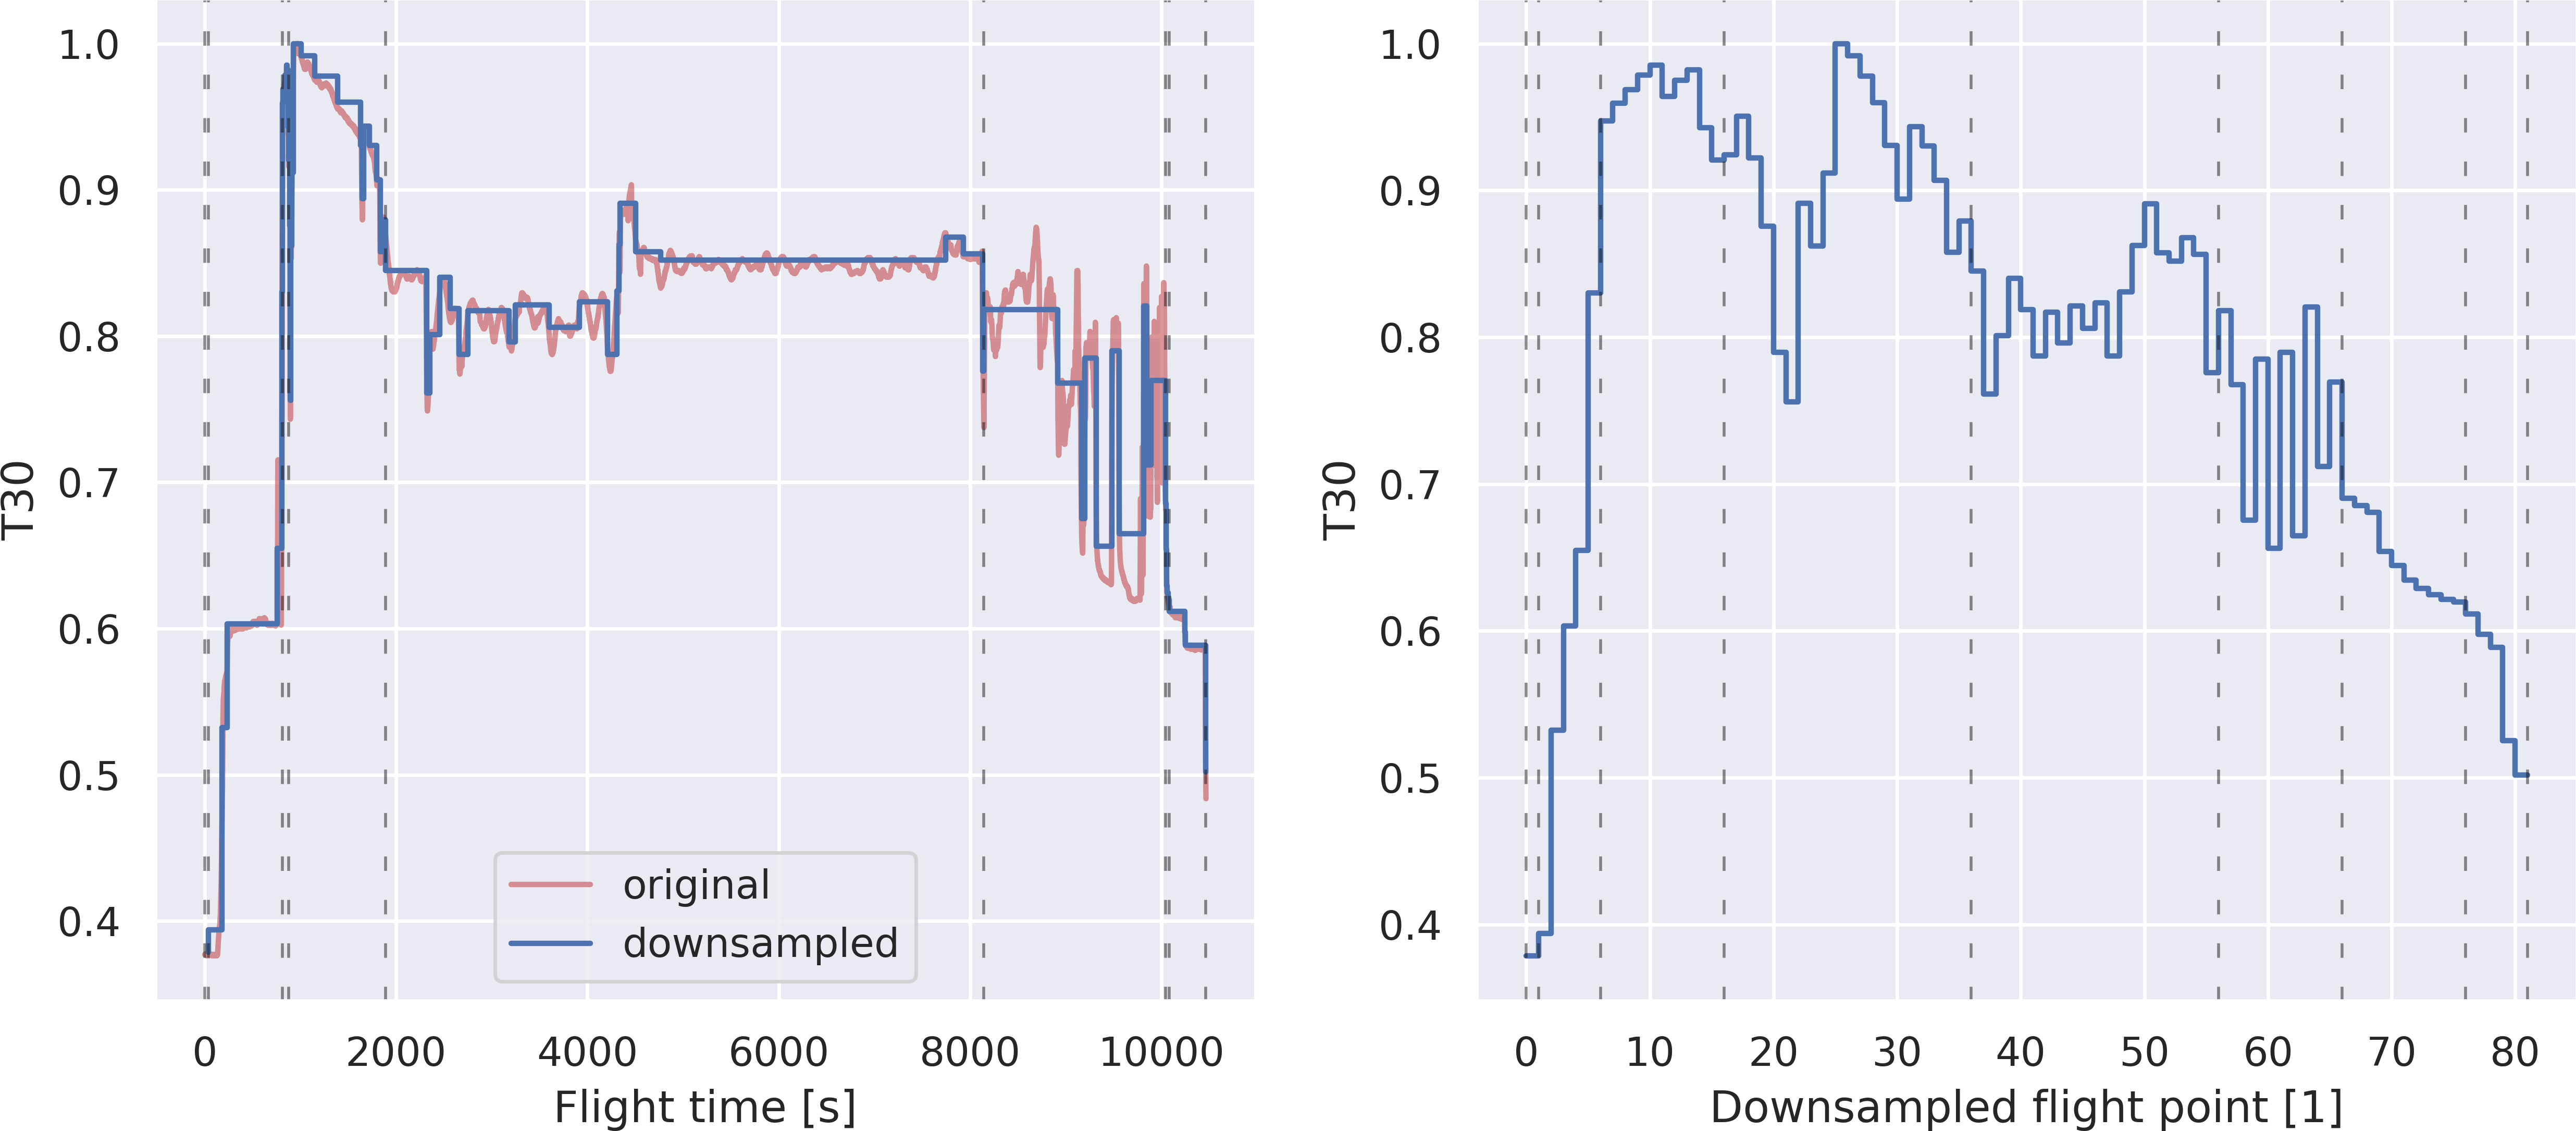
\includegraphics[width=\textwidth]{0815_ds}
    \caption{\label{fig:0815_ds} \textbf{Left:} Downsampled parameter T30 of Flight 0815 (81 data points) compared to the original time series (10\,466 data points). \textbf{Right:} Downsampled values alone with equal spacing in the \(x\)-direction. All parameter values normalised.}
\end{figure}

The second reason for downsampling data is the computational benefit of having significantly less information to process. Downsampling can help to remove noise from data which is otherwise computationally costly while offering no additional information of value. In total, the volume of flight data was reduced by 99.2\%, which enabled an equivalent improvement in computation time for models with a complexity of \(O(n)\) (where \(n\) is the number of input values), such as those based on InceptionTime \cite[]{fawaz_inceptiontime_2019}.

Each channel of each flight's \ac{mts} was approximated to fixed-length flight phases. The output for each channel was a time series of 81 values that approximate the flight parameter with minimal reconstruction error. The flight phases described in Table \ref{tab:flight_phases} were reduced to the corresponding number of values from the column `Downsampled length'. These values were determined based on a combination of the corresponding phase's relevance to damage (e.g. take-off generally contains peak values that have a great influence on damage) and its average length relative to the rest of the flight (e.g. cruise).

Two visualisations of the downsampled T30 time series from Flight 0815 is shown in Figure \ref{fig:0815_ds}.

\subsubsection{Reconstruction Error} \label{sec:recon_err}
The term \textit{reconstruction error} refers to the amount of information lost due to downsampling. This can be quantified in several ways, but is essentially some form of distance between the original data and its approximation.

Given the original time series, \(Q = \left[q_1,\,\ldots,\,q_m\right]\) and its downsampled representation \(R = \left[r_1,\,\ldots,\,r_n\right]\), \(m > n\), one simple measure for reconstruction error is given by

\[
    D(Q,\,R') = \frac{1}{m}\sum_{i=1}^{m}{q_i - r'_i}
\]

where \(i \in \left[1,\,m\right]\), and where \(R'\) (and its elements \(r'_i\)) represent a transformed \(R\) in which the downsampled values are repeated until the index of the next downsampled value is reached, such that \(R'\) contains as many values as \(Q\) (\(m\) in total) and that \(R'\) can be subtracted element-wise from \(Q\).

Based on this measure, the reconstruction error of the downsampled data is 1.2\%, or an average deviation of 0.012 from the original per data point, which is not expected to cause issues in terms of data loss. However, particularly during the descent phase, as is visible in Figure \ref{fig:0815_ds}, many of the peaks and troughs are lost to the algorithm. Since these occur within a low range relative to the maximum where impact on damage is less significant, it is not expected that the information lost be of great value.

\subsubsection{Visualisation}
With the flights in a uniform, downsampled representation, some characteristics of the data begin to become more apparent.

\paragraph{NH}
\begin{figure}
    \centering
    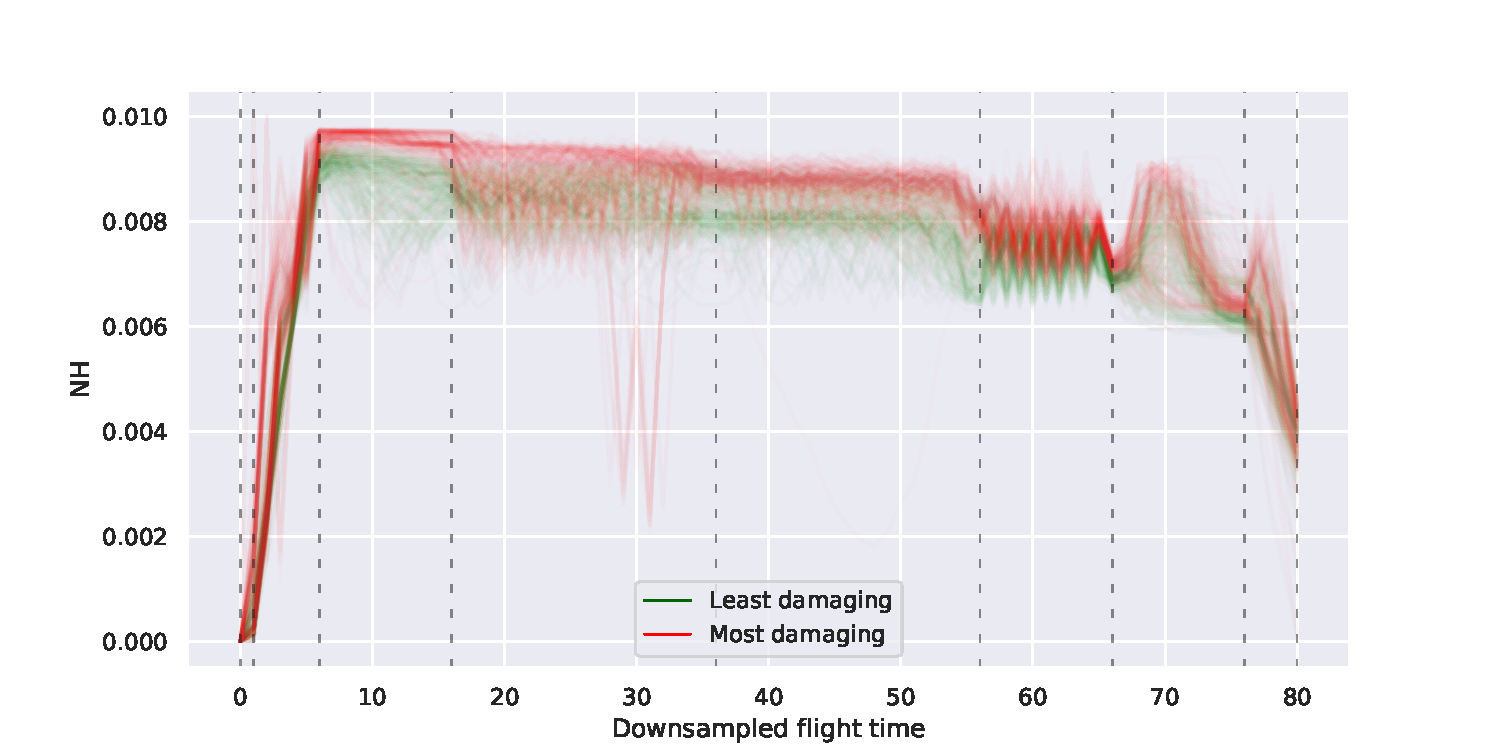
\includegraphics[width=\textwidth]{f3_NH_high_low_dmg_500}
    \caption{\label{fig:high_low_dmg_NH} Line plot showing NH from 500 flights, coloured according to their damage to feature 3. Red lines represent the 250 flights with the most damage to this feature, green the 250 with the least. All parameter values normalised.}
\end{figure}

To create Figure \ref{fig:high_low_dmg_NH}, the flights were ordered by damage at feature 3. From these, the 250 flights with the lowest damage (fewer than 0.53 cycles) and the 250 with the highest damage (more than 1.15 cycles) were extracted. The NH curves of these 500 flights were plotted at low opacity over one another.

\begin{figure}
    \centering
    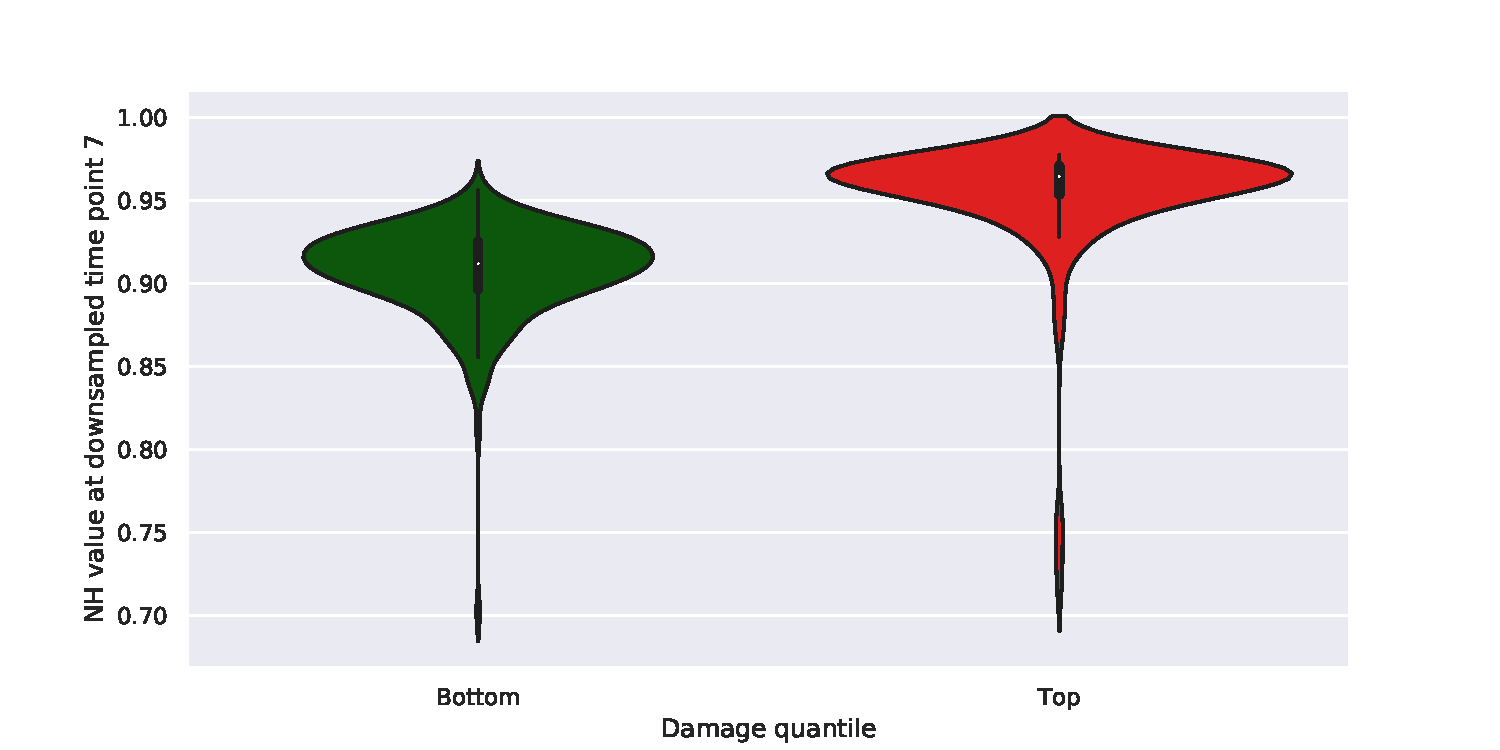
\includegraphics[width=\textwidth]{f3_NH_high_low_dmg_500_dist_t7}
    \caption{\label{fig:dmg_violin_NH} Violin plot showing the distribution of NH values at downsampled time point 7, coloured according damage to feature 3. All parameter values normalised.}
\end{figure}

This representation shows a clear (albeit unsurprising) separation of high- and low-damage flights across the entire range, with a particularly clear gap around downsampled time point 7 --- an early point during the take-off phase where NH generally peaks --- and gives an idea of one type of characteristic that the neural networks should be able to learn. Figure \ref{fig:dmg_violin_NH} shows the distribution of NH values at time point 7 for feature 3. The boxplots contained within the so-called violins show that the majority of these flights could be categorised correctly as high- or low-damage based on this single time point. If the NH value towards the beginning of take-off is below 0.94, it is most likely to be a low-damage flight; if above, a high-damage flight.

\paragraph{ALT}
Figure \ref{fig:high_low_dmg_ALT} shows the sensitivity of feature 2 to altitude. The higher the flight altitude, the higher the damage. The reason for this is atmospheric pressure: At high altitudes, the rotational speed of the fan must be increased to compensate for the lack of air (and therefore oxygen) for combustion. This claim is supported by the sensitivity of features 1 and 2 to altitude (Figures \ref{fig:dmg_violin_ALT_f1} and \ref{fig:dmg_violin_ALT_f2}) as these were expected to be sensitive to NH (Section \ref{sec:features}). This is a strong contrast to the relative indifference to altitude of, for example, feature 6 (Figure \ref{fig:dmg_violin_ALT_f6}).

\begin{figure}
    \centering
    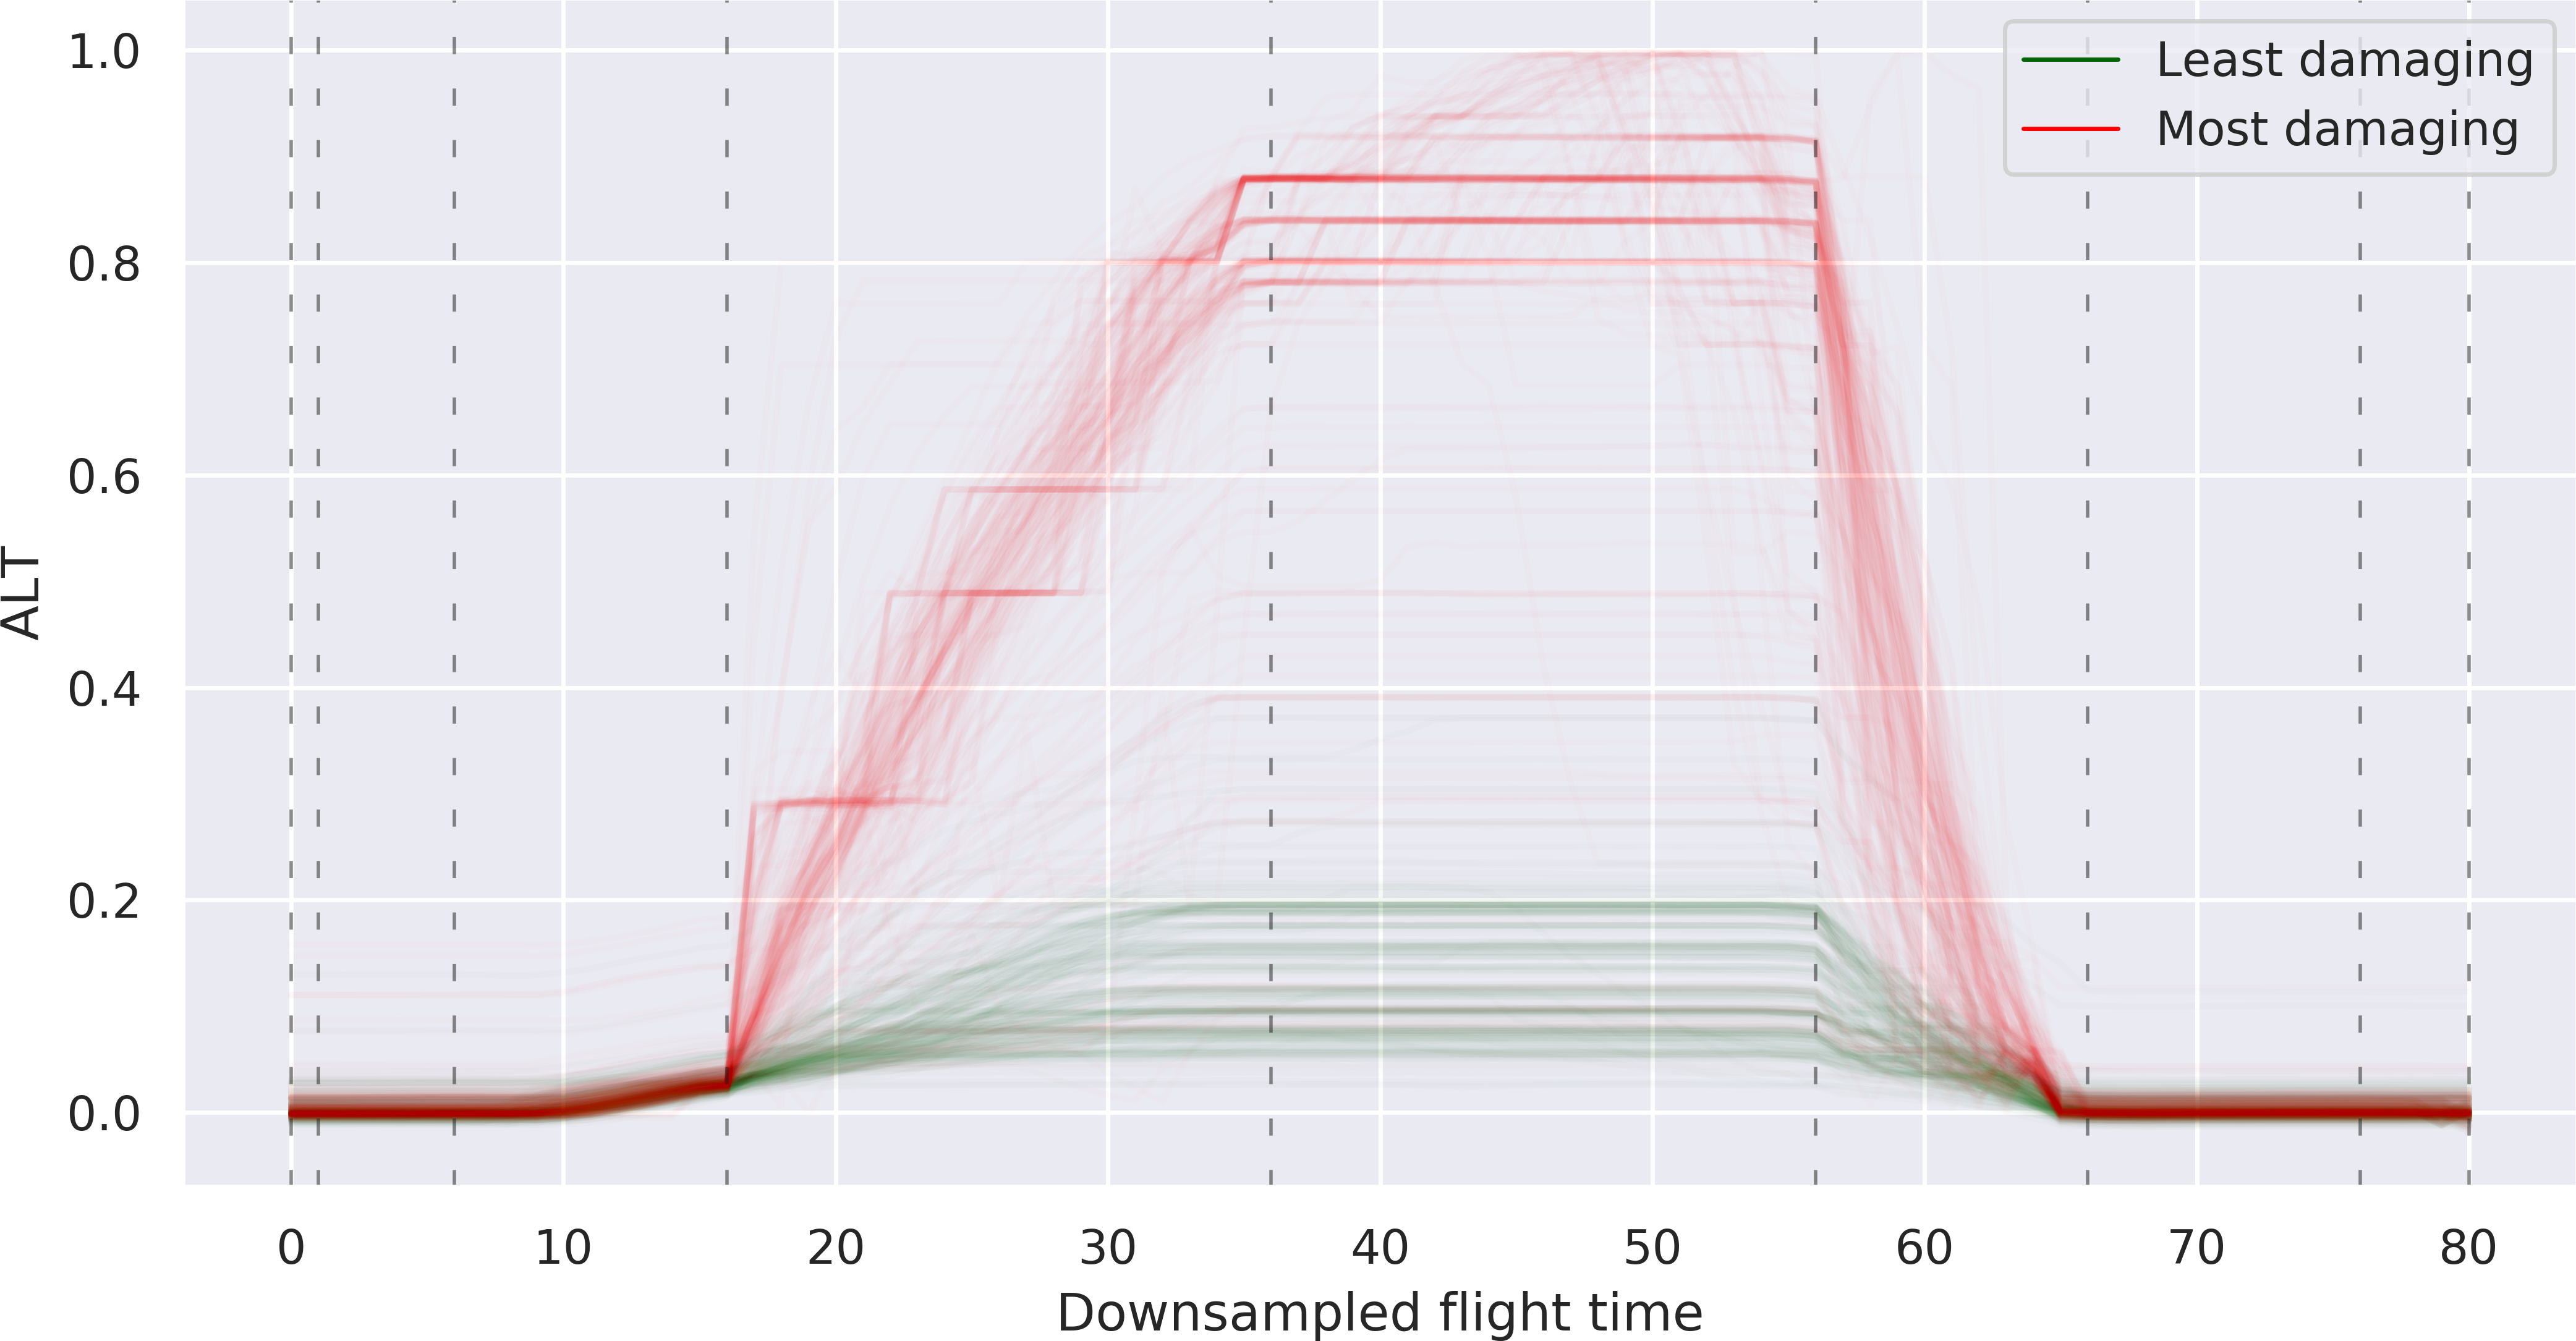
\includegraphics[width=\textwidth]{f2_ALT_high_low_dmg_500}
    \caption{\label{fig:high_low_dmg_ALT} Line plot showing ALT from 500 flights, coloured according to their damage to feature 1. Red lines represent the 250 flights with the most damage to this feature, green the 250 with the least. All parameter values normalised.}
\end{figure}

\begin{figure}
    \centering
    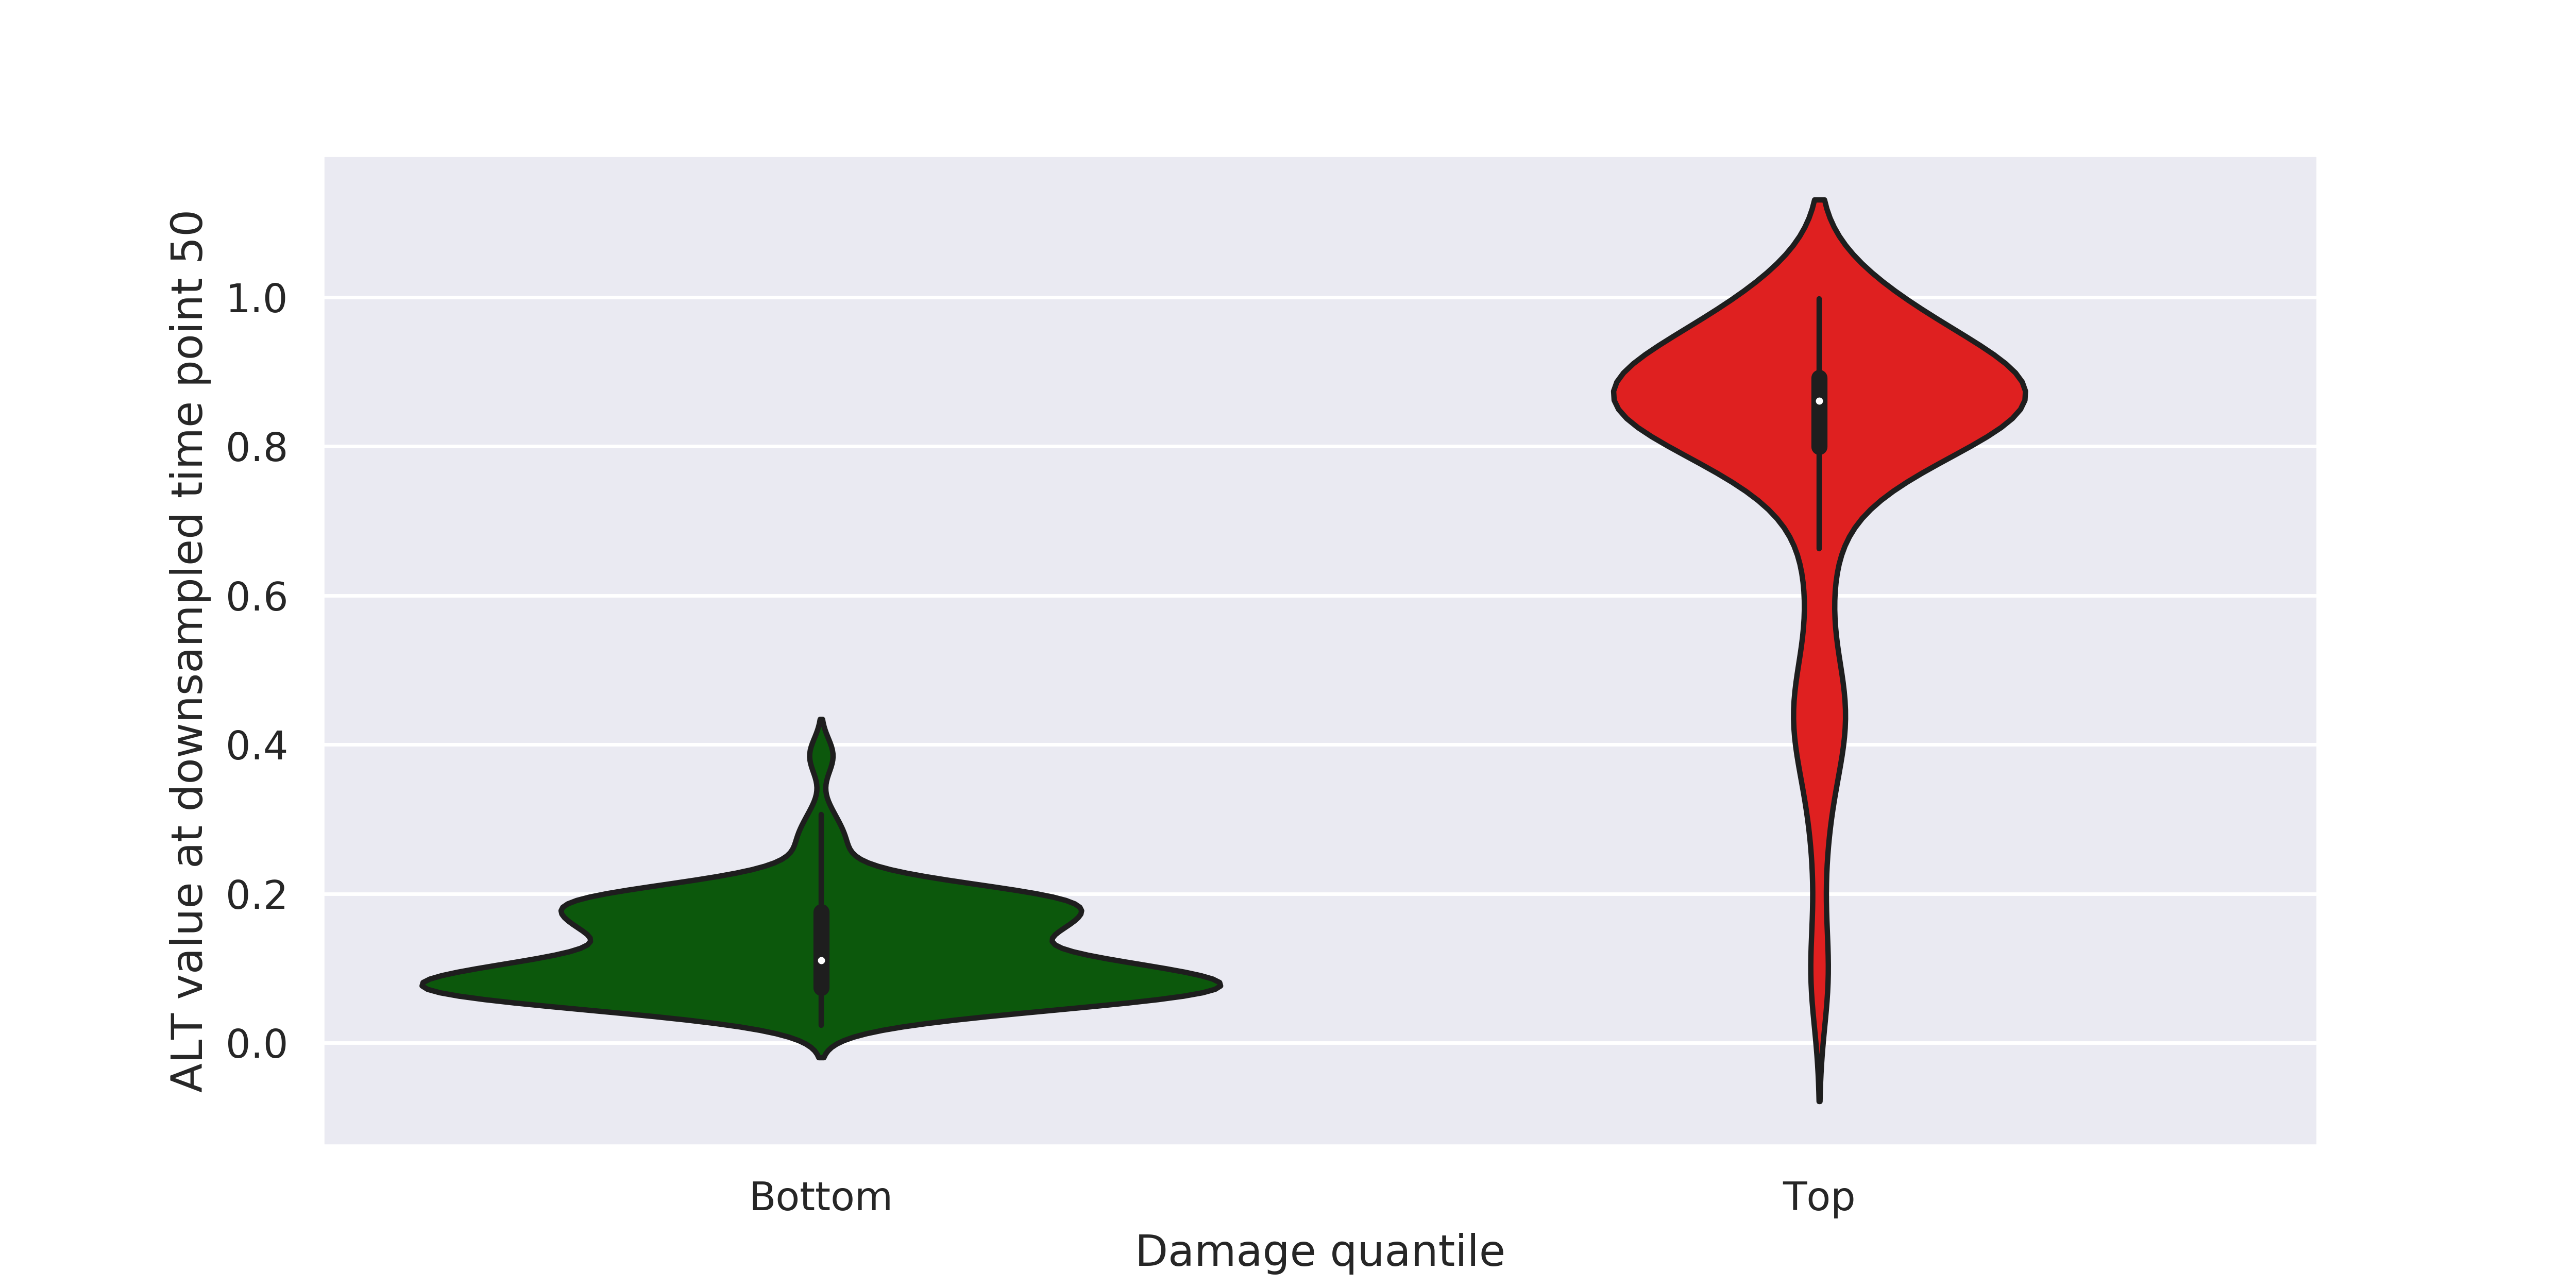
\includegraphics[width=\textwidth]{f1_ALT_high_low_dmg_500_dist_t50}
    \caption{\label{fig:dmg_violin_ALT_f1} Violin plot showing the distribution of ALT values at downsampled time point 50 (middle of cruise phase), coloured according to damage to feature 1. All parameter values normalised.}
\end{figure}

\begin{figure}
    \centering
    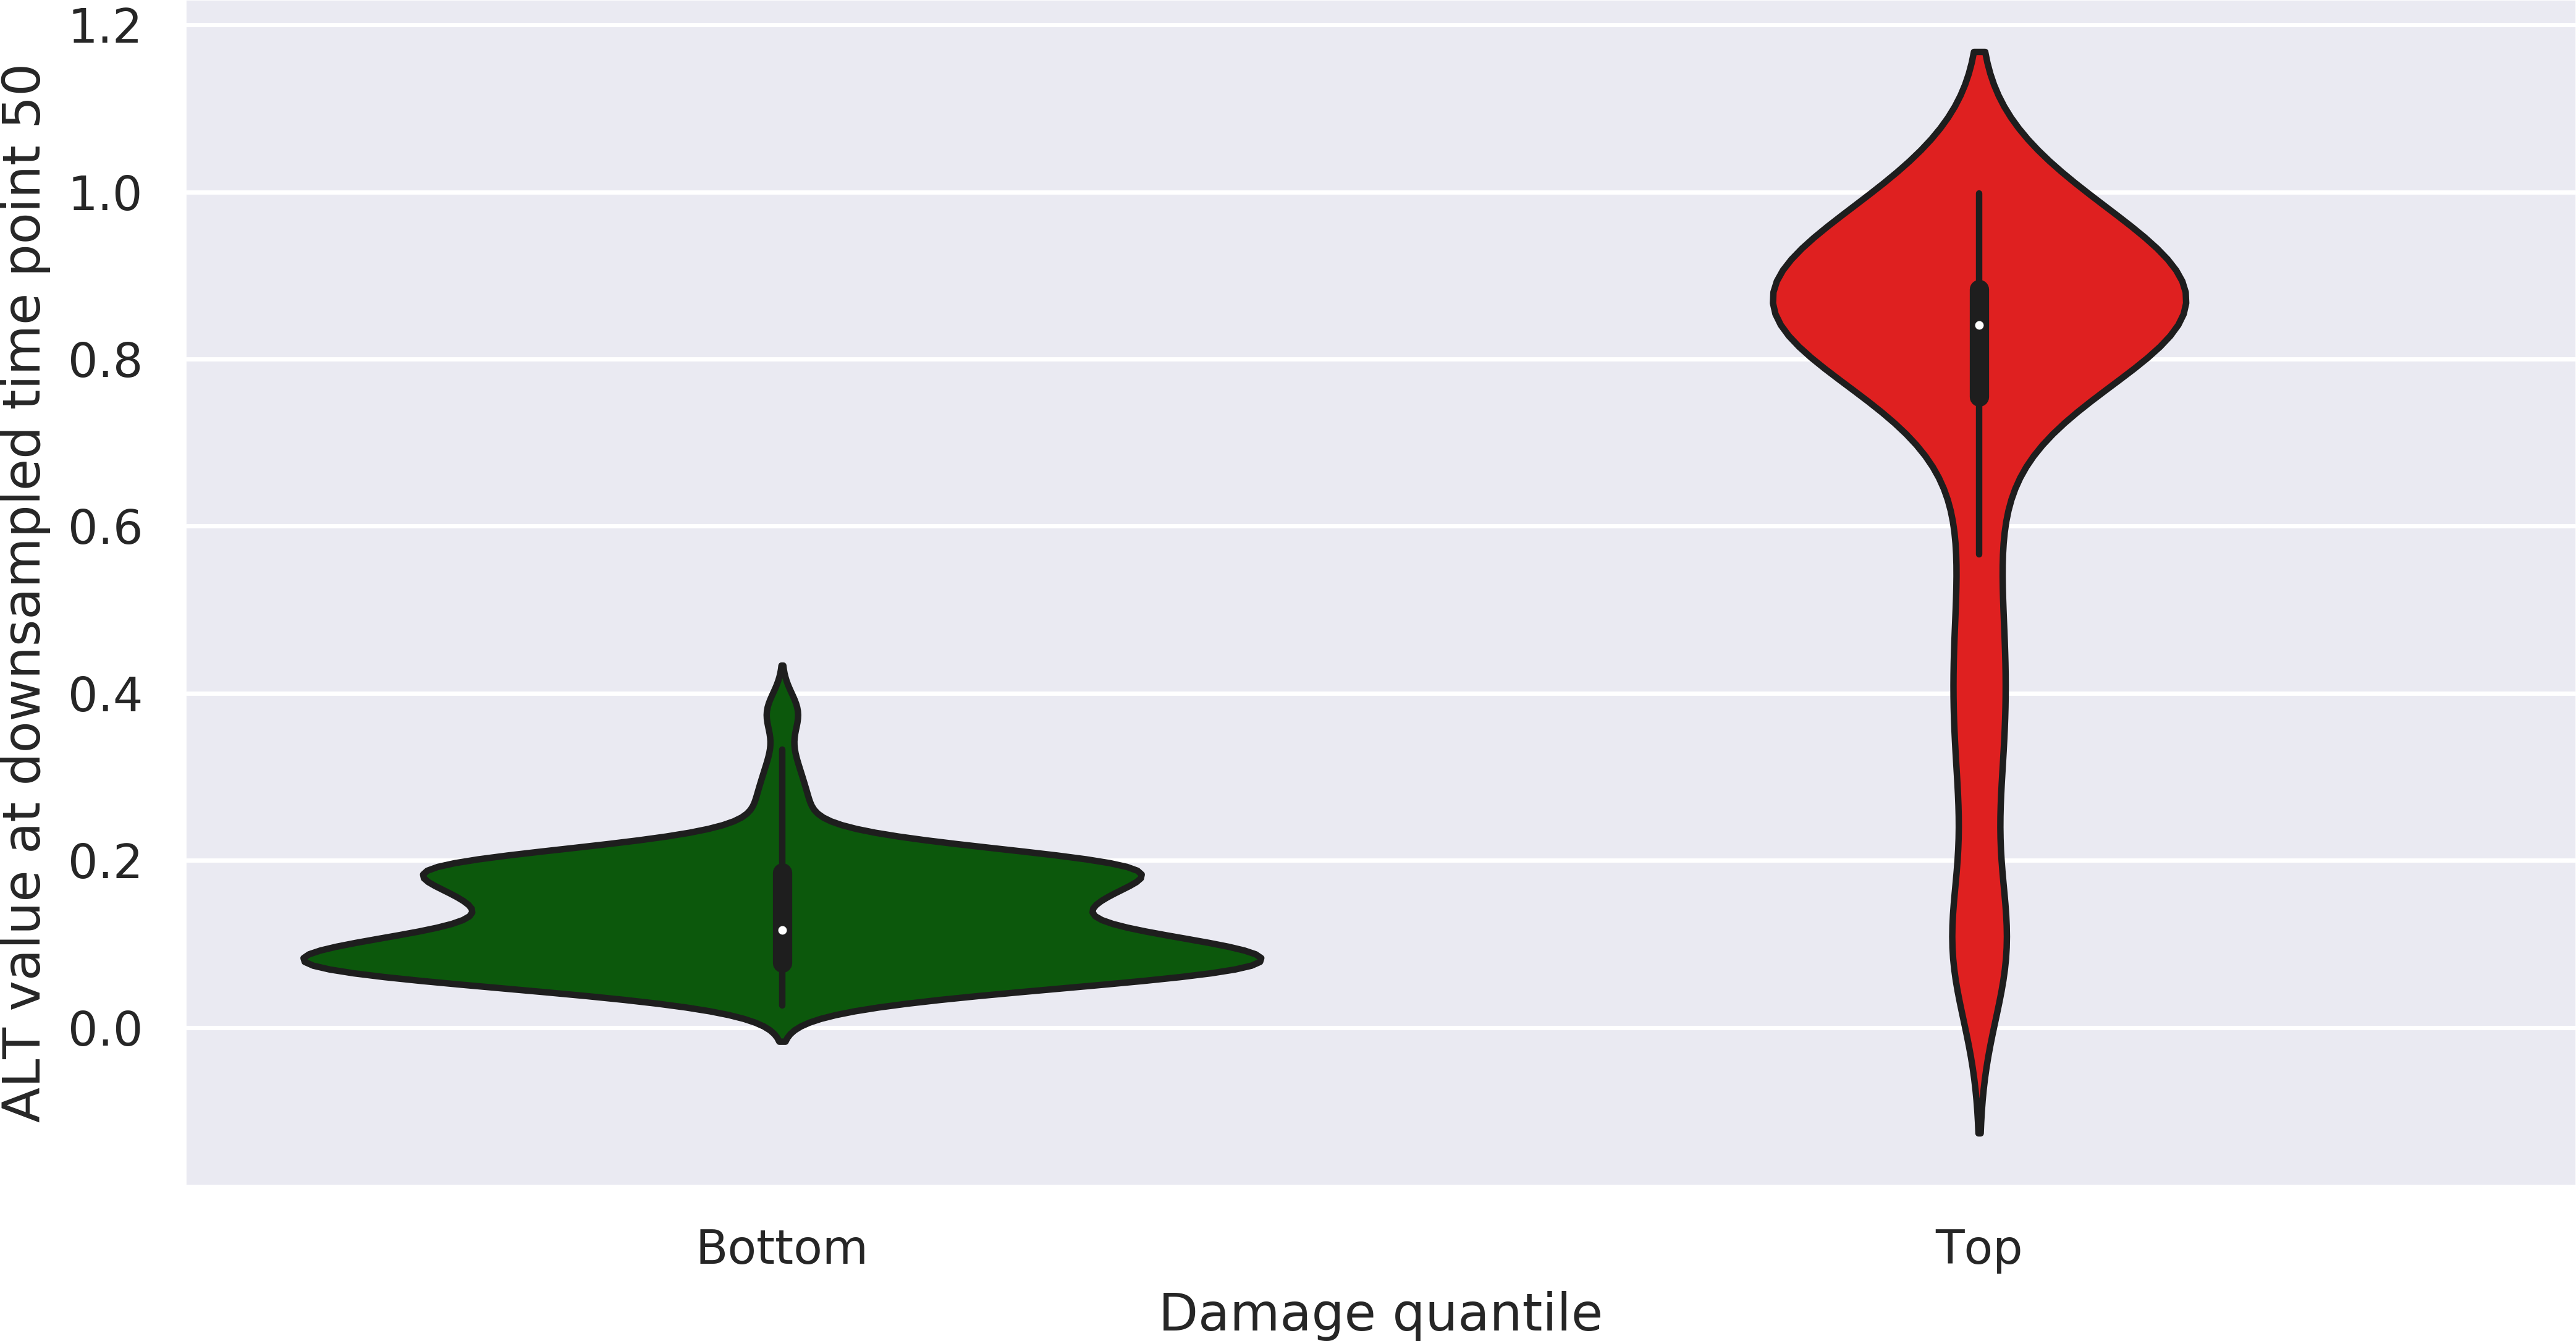
\includegraphics[width=\textwidth]{f2_ALT_high_low_dmg_500_dist_t50}
    \caption{\label{fig:dmg_violin_ALT_f2} Violin plot showing the distribution of ALT values at downsampled time point 50 (middle of cruise phase), coloured according to damage to feature 2. All parameter values normalised.}
\end{figure}

\begin{figure}
    \centering
    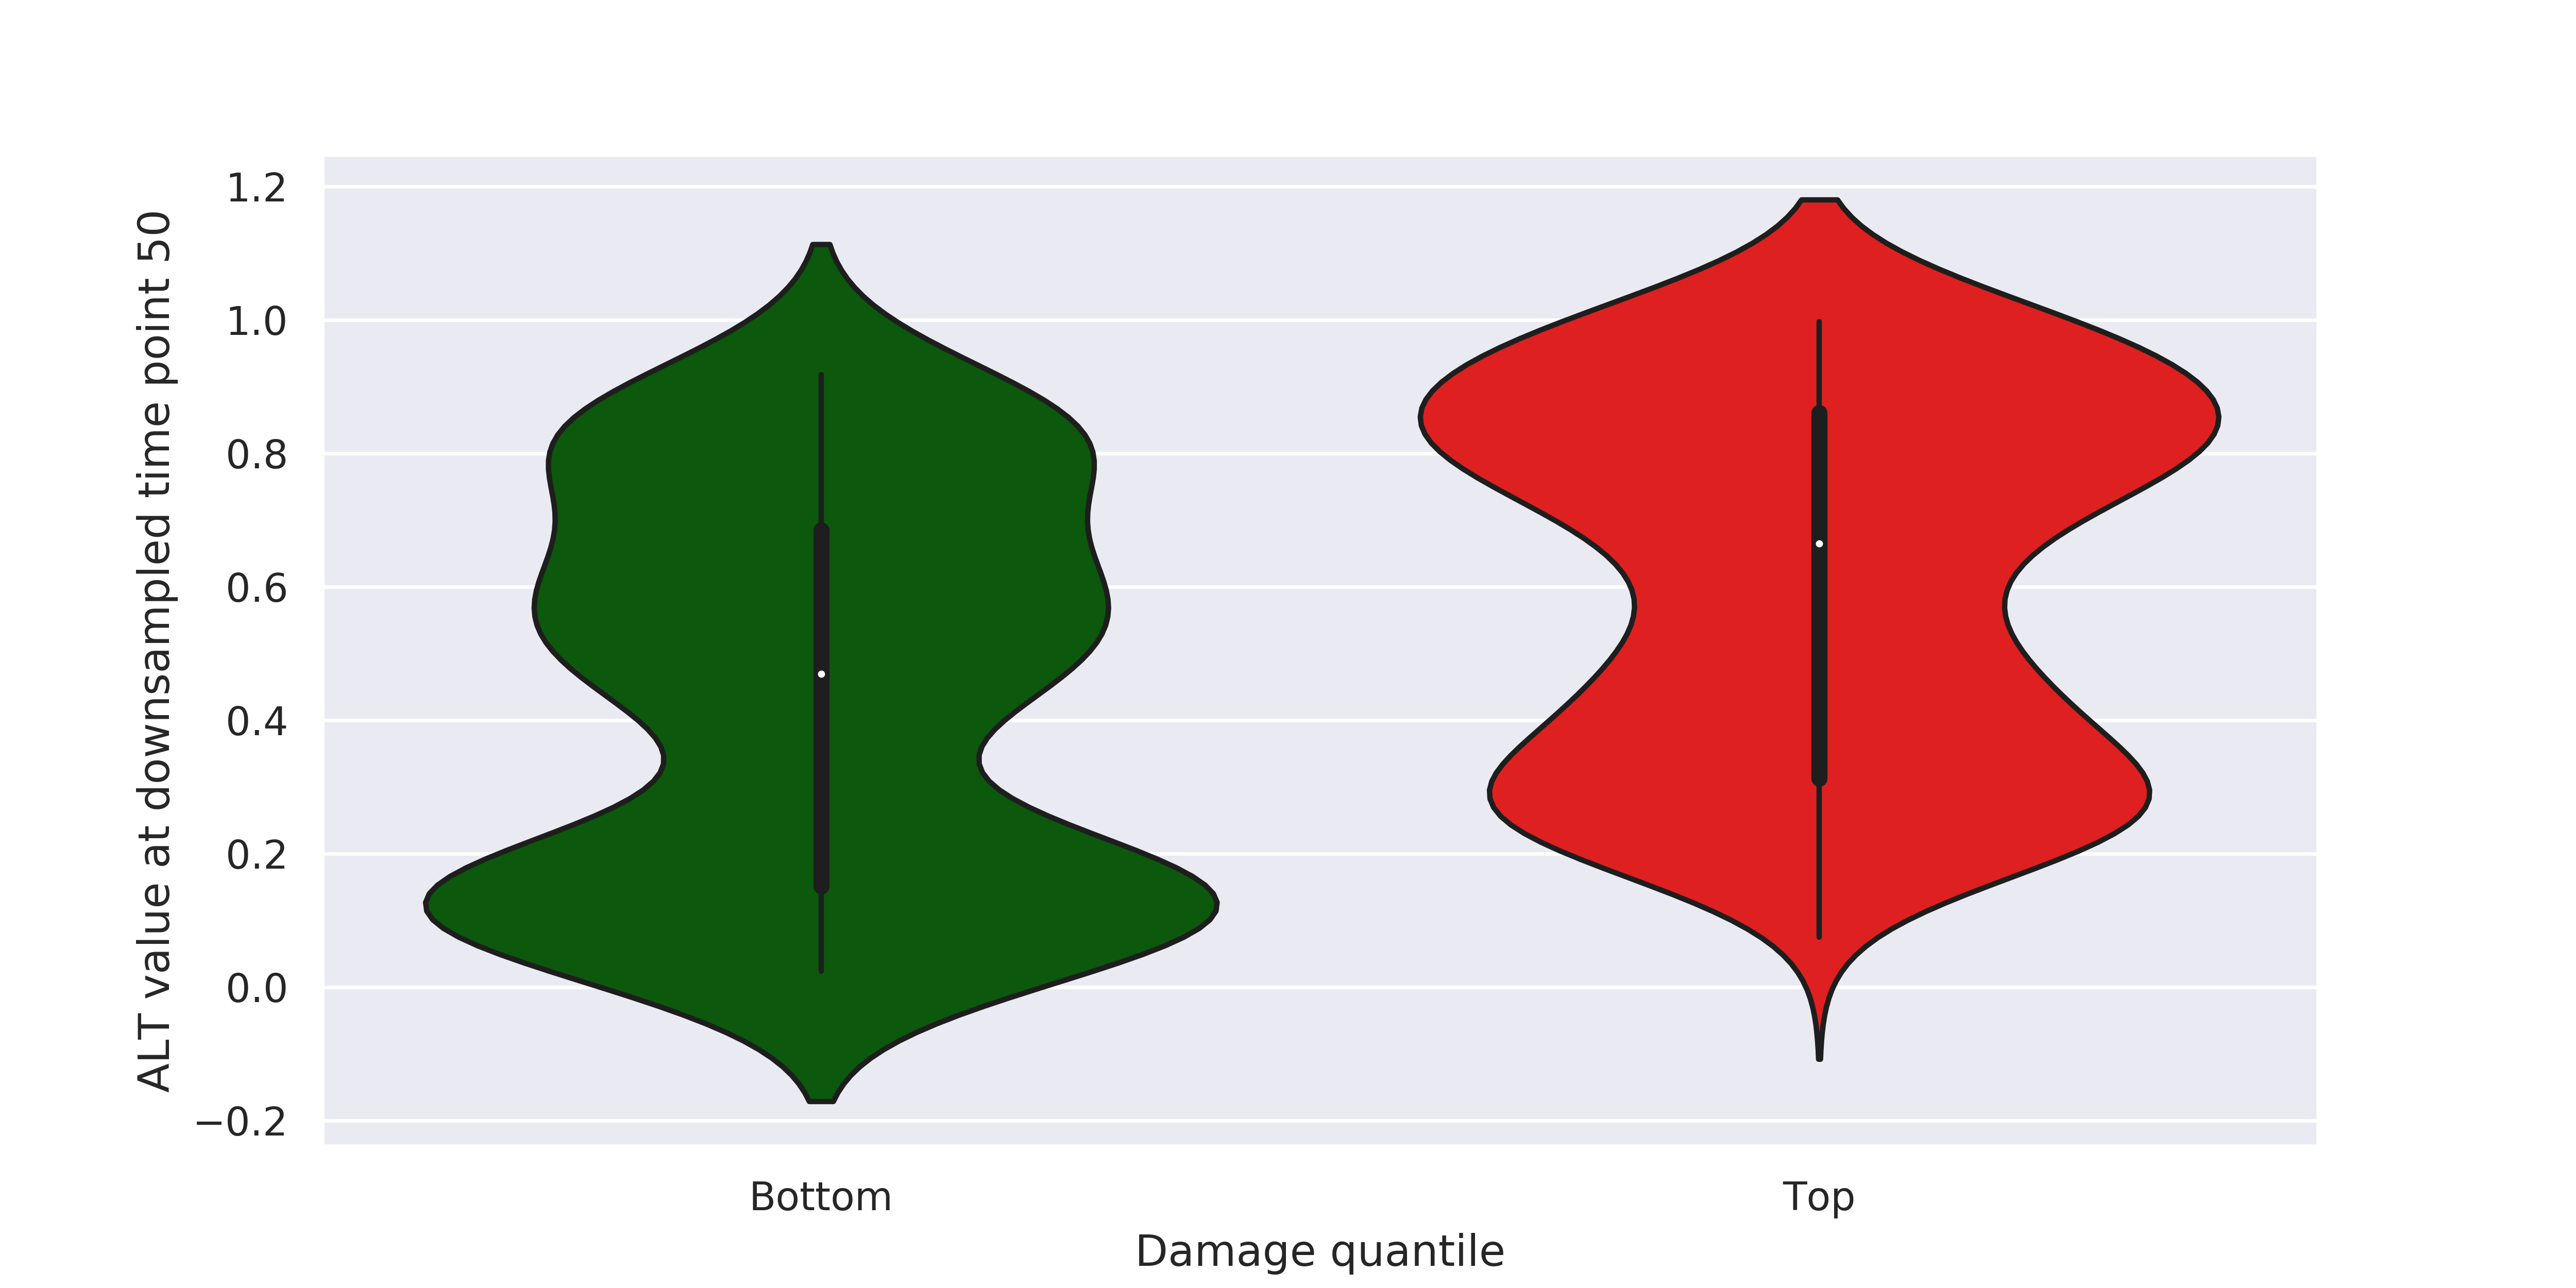
\includegraphics[width=\textwidth]{f6_ALT_high_low_dmg_500_dist_t50}
    \caption{\label{fig:dmg_violin_ALT_f6} Violin plot showing the distribution of ALT values at downsampled time point 50 (middle of cruise phase), coloured according to damage to feature 6. All parameter values normalised.}
\end{figure}

\paragraph{P30}
Figure \ref{fig:high_low_dmg_P30} shows P30 values for feature 5. As expected, a higher peak pressure during the take-off phase causes a higher consumption of service life. During the cruise phase, a vague tendency in the opposite direction --- lower pressure, higher damage --- is visible. This, as with altitude, can be attributed to altitude, where a lower atmospheric pressure causes an increase in rotational speed.

\begin{figure}
    \centering
    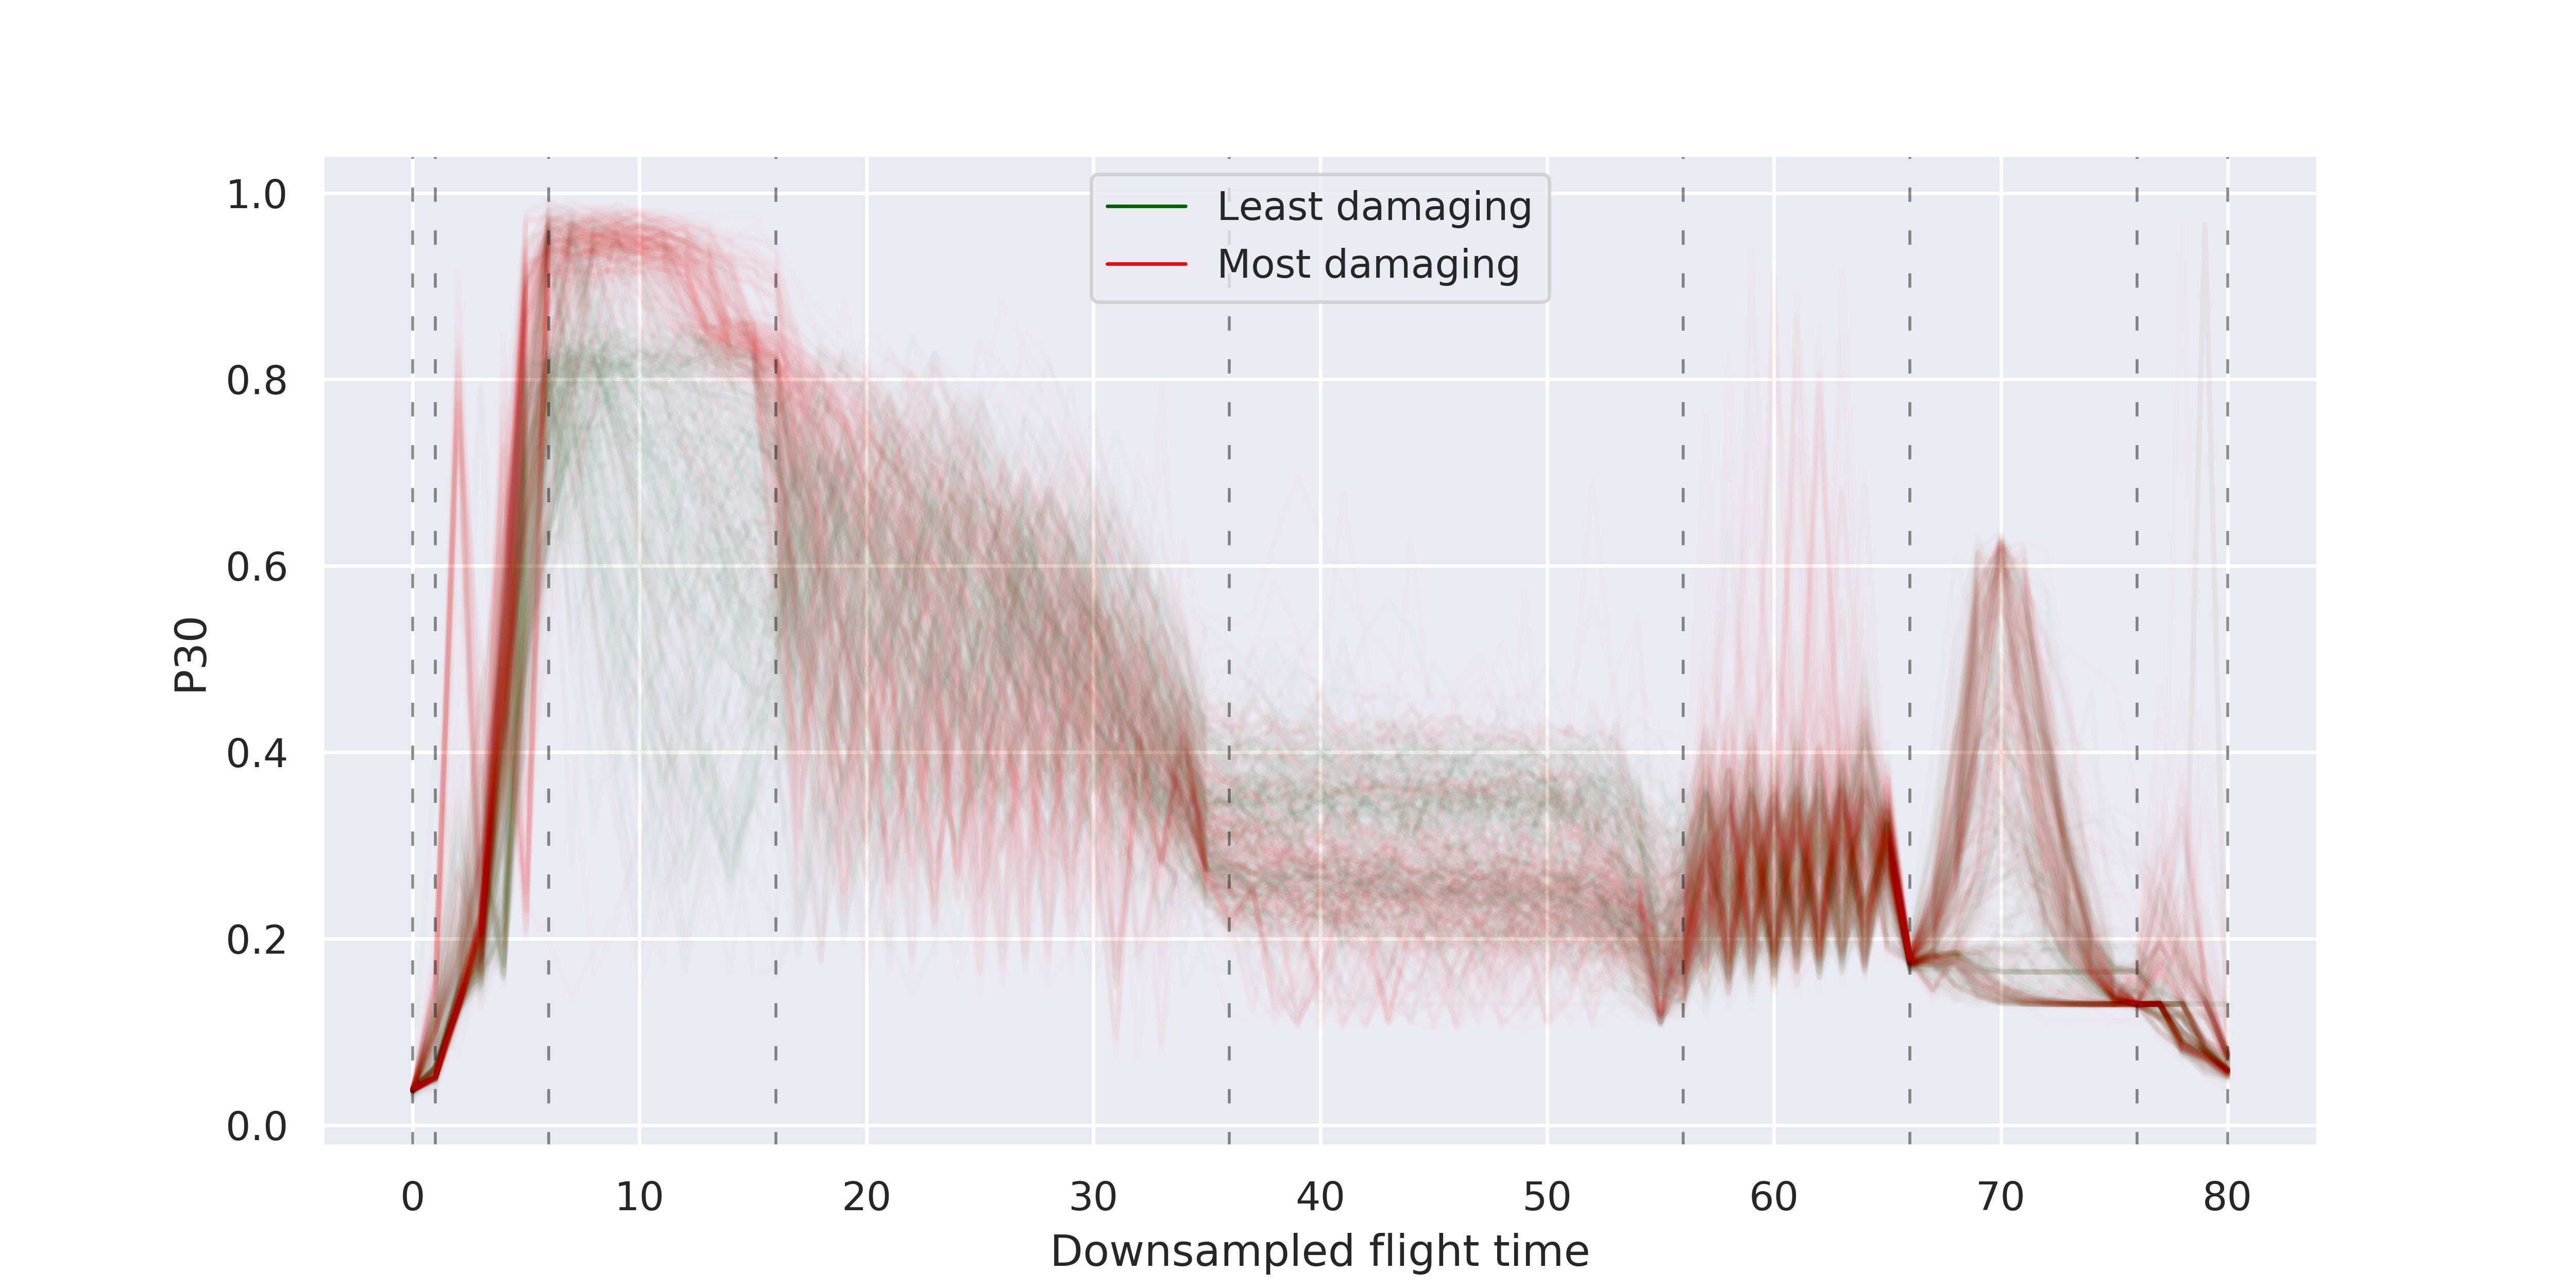
\includegraphics[width=\textwidth]{f5_P30_high_low_dmg_500}
    \caption{\label{fig:high_low_dmg_P30} Line plot showing P30 from 500 flights, coloured according to their damage to feature 5. Red lines represent the 250 flights with the most damage to this feature, green the 250 with the least. All parameter values normalised.}
\end{figure}

% Figure \ref{fig:f1_dmg_violin} shows a violin plot of P30 values at time point 36 --- the first point of the cruise phase. While the difference in distribution here is not as significant as in Figure \ref{fig:f3_dmg_violin} (as shown by the overlapping inner quantiles of the boxplots), there

% \begin{figure}
%     \centering
%     \includegraphics[width=\textwidth]{high_low_dmg/P30/f1_P30_high_low_dmg_500_dist_t36}
%     \caption{\label{fig:f1_dmg_violin} Violin plot showing the distribution of P30 values at downsampled time point 36, coloured according damage to feature 1. All parameter values normalised.}
% \end{figure}

% T30
\paragraph{T30}
\begin{figure}
    \centering
    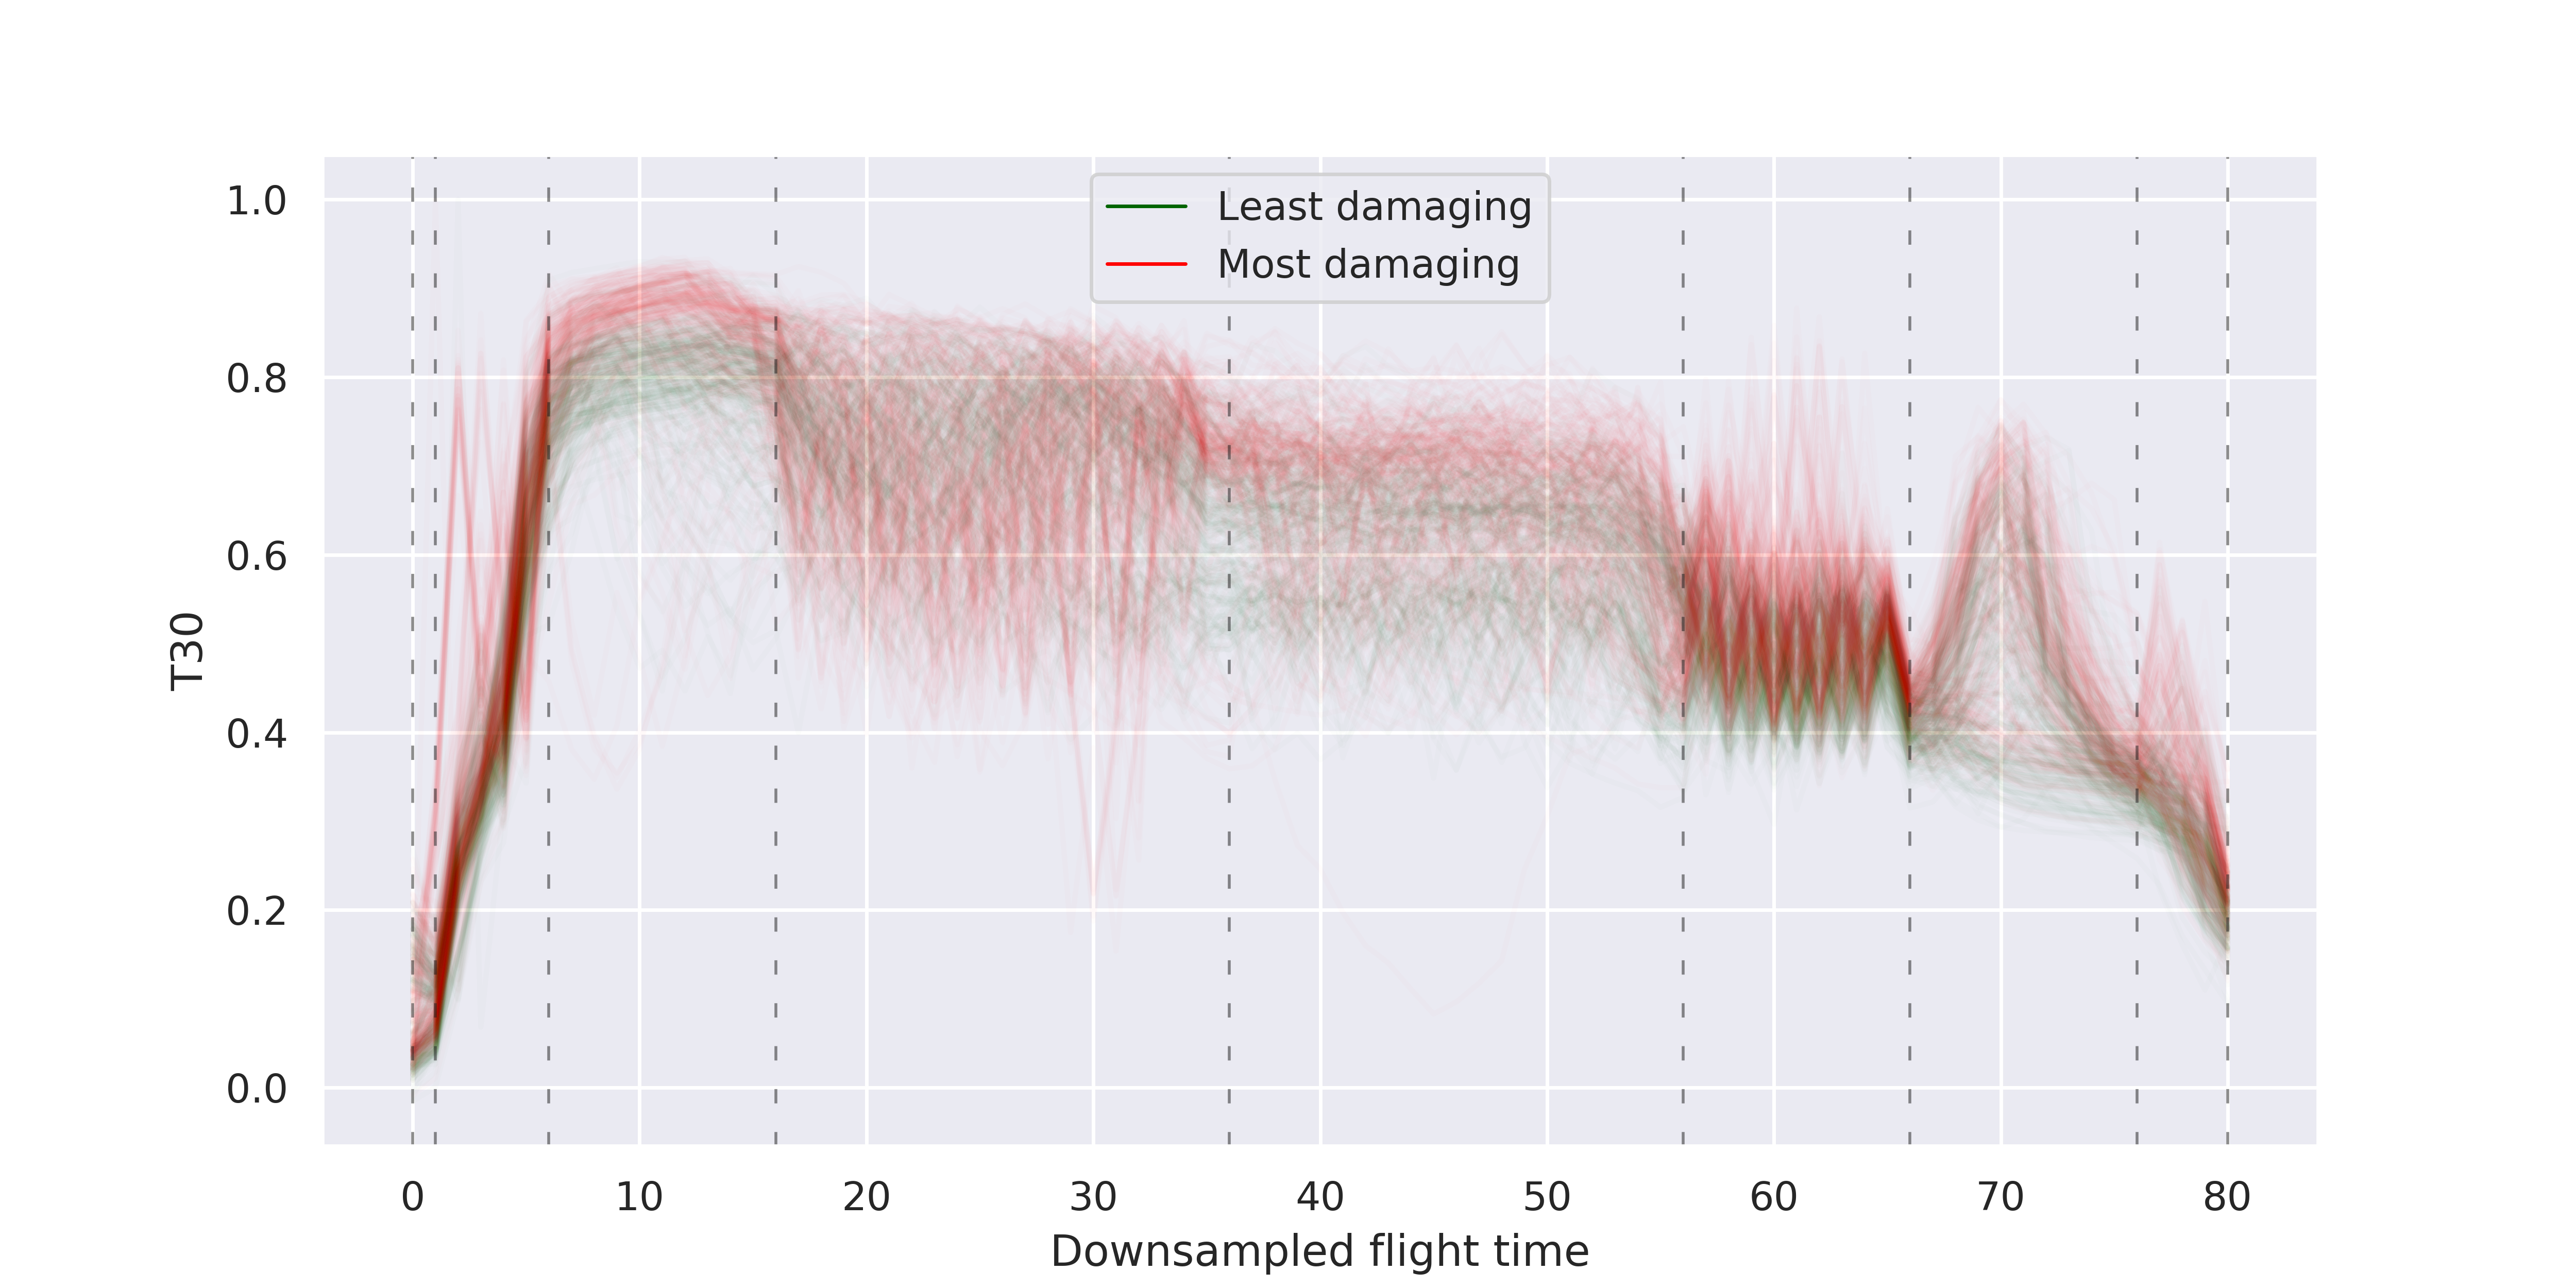
\includegraphics[width=\textwidth]{f6_T30_high_low_dmg_500}
    \caption{\label{fig:high_low_dmg_T30} Line plot showing T30 from 500 flights, coloured according to their damage to feature 6. Red lines represent the 250 flights with the most damage to this feature, green the 250 with the least. All parameter values normalised.}
\end{figure}

As well as the expected influence of peak temperature at during take-off, Figure \ref{fig:high_low_dmg_T30} shows a tendency during the climb phase for high damage if large fluctuations are present, as shown by the sharp, downwards-pointing, red V-shaped lines between T30 values of approximately 0.4 and 0.85. Since this flight characteristic can occur at any point during the climb, this is the type of value progression that should be picked up by filters in a \ac{cnn}.

\subsection{Dataset Reduction} \label{sec:data_sizes}
The complete dataset consists of \ac{ehm} data for 14\,045 flights, as well as seven Cycle Counter output values for each flight. Since scalability is an important factor in the research, the dataset was separated into two further datasets of 4\,213 and 1\,211 flights in order to test model performance on smaller training datasets. (These three datasets will hereinafter be referred to as `complete', `reduced' and `greatly reduced', respectively.)

These datasets were further split into training and validation subsets at a ratio of 3:1 (before rounding). The complete dataset therefore consisted of 10\,534 training and 3\,511 validation flights, the reduced dataset 3\,160 and 1\,053, and the greatly reduced dataset 909 and 302. The flights numbers in each set and subset were kept constant throughout all models to avoid skewing the data.

% \subsection{Optional: Case Studies}

% \subsubsection{6014: Stress Ranges}

% \subsubsection{6079: Long Taxi}